% `template.tex', a bare-bones example employing the AIAA class.
%
% For a more advanced example that makes use of several third-party
% LaTeX packages, see `advanced_example.tex', but please read the
% Known Problems section of the users manual first.
%
% Typical processing for PostScript (PS) output:
%
%  latex template
%  latex template   (repeat as needed to resolve references)
%
%  xdvi template    (onscreen draft display)
%  dvips template   (postscript)
%  gv template.ps   (onscreen display)
%  lpr template.ps  (hardcopy)
%
% With the above, only Encapsulated PostScript (EPS) images can be used.
%
% Typical processing for Portable Document Format (PDF) output:
%
%  pdflatex template
%  pdflatex template      (repeat as needed to resolve references)
%
%  acroread template.pdf  (onscreen display)
%
% If you have EPS figures, you will need to use the epstopdf script
% to convert them to PDF because PDF is a limmited subset of EPS.
% pdflatex accepts a variety of other image formats such as JPG, TIF,
% PNG, and so forth -- check the documentation for your version.
%
% If you do *not* specify suffixes when using the graphicx package's
% \includegraphics command, latex and pdflatex will automatically select
% the appropriate figure format from those available.  This allows you
% to produce PS and PDF output from the same LaTeX source file.
%
% To generate a large format (e.g., 11"x17") PostScript copy for editing
% purposes, use
%
%  dvips -x 1467 -O -0.65in,0.85in -t tabloid template
%
% For further details and support, read the Users Manual, aiaa.pdf.


% Try to reduce the number of latex support calls from people who
% don't read the included documentation.
%


\typeout{}\typeout{If latex fails to find aiaa-tc, read the README file!}
%


\documentclass[]{aiaa-tc}% insert '[draft]' option to show overfull boxes
\usepackage{float}
\usepackage{epstopdf}

\title{ASEN 5070 Project}

\author{
	Johnathan Clouse%
	\thanks{Graduate Students, Aerospace Engineering Sciences, 1111 Engineering Drive, Boulder, CO, 80309-0429}\\
	{\normalsize\itshape
		University of Colorado, Boulder, CO, 80309-0429, USA}
}

% Define commands to assure consistent treatment throughout document
\newcommand{\eqnref}[1]{(\ref{#1})}
\newcommand{\class}[1]{\texttt{#1}}
\newcommand{\package}[1]{\texttt{#1}}
\newcommand{\file}[1]{\texttt{#1}}
\newcommand{\BibTeX}{\textsc{Bib}\TeX}

\usepackage[euler]{textgreek}
\usepackage[colorlinks=true]{hyperref}
\hypersetup{urlcolor=cyan}

\usepackage{listings}
\usepackage{color} %red, green, blue, yellow, cyan, magenta, black, white
\definecolor{mygreen}{RGB}{28,172,0} % color values Red, Green, Blue
\definecolor{mylilas}{RGB}{170,55,241}

\usepackage{tablefootnote}
\usepackage{graphicx}
\usepackage{amsmath}
\usepackage{bm}
\usepackage{subfigure}
%\usepackage{subcaption}

\definecolor{mylilas}{RGB}{170,55,241}

% See p.105 of "TeX Unbound" for suggested values.
% See pp. 199-200 of Lamport's "LaTeX" book for details.
%   General parameters, for ALL pages:
\renewcommand{\topfraction}{0.9}	% max fraction of floats at top
\renewcommand{\bottomfraction}{0.8}	% max fraction of floats at bottom
%   Parameters for TEXT pages (not float pages):
\setcounter{topnumber}{2}
\setcounter{bottomnumber}{2}
\setcounter{totalnumber}{4}     % 2 may work better
\setcounter{dbltopnumber}{2}    % for 2-column pages
\renewcommand{\dbltopfraction}{0.9}	% fit big float above 2-col. text
\renewcommand{\textfraction}{0.07}	% allow minimal text w. figs
%   Parameters for FLOAT pages (not text pages):
\renewcommand{\floatpagefraction}{0.7}	% require fuller float pages
% N.B.: floatpagefraction MUST be less than topfraction !!
\renewcommand{\dblfloatpagefraction}{0.7}	% require
    \makeatletter
    \renewcommand\l@section{\@dottedtocline{2}{1.5em}{3em}}
    \makeatother
    
\begin{document}
	

	
	\maketitle
	
	\begin{abstract}
		\noindent 
		
	\end{abstract}
	
	\newpage
	
	\tableofcontents
	
	\newpage
	
	\section{The Orbit Determination Problem}
	
	 The process of orbit determination is one that combines observations and known dynamics to produce the most likely state of a satellite body in some reference frame.  By creating and propagating a reference state based on \textit{a priori} information, one can estimate the deviation from the reference state such that the estimated state is the best fit with observations. If the reference state is sufficiently close to the true state, the problem can be linearized to map the states from epoch to epoch.  This problem becomes nontrivial in the presence of perturbations due to gravity fields, drag, third bodies, etc.  Born et al. is the primary source for the formulations that follow.
	
	\vspace{5 mm}
	
	 The following equations define the variables needed to linearize the orbit determination problem
	\begin{equation}
	\begin{matrix}
	\mathbf{x}(t)=\mathbf{X}(t)-\mathbf{X}^{*}(t) \\
	\mathbf{y}(t)=\mathbf{Y}(t)-\mathbf{Y}^{*}(t)=G(\mathbf{X},t)+\boldsymbol{\epsilon}-G(\mathbf{X}^{*},t)
	\end{matrix}
	\end{equation}

	\noindent where $\mathbf{X}(t)$ is the true state, $\mathbf{X}^{*}(t)$ is the propagated reference state, and $\mathbf{x}(t)$ is the deviation between the two. For the observations, $\mathbf{Y}(t)$ represents the measurements taken of the state, $\mathbf{Y}^{*}(t)$ is the computed measurements from $\mathbf{X}^{*}(t)$ at the same time, and $\mathbf{y}(t)$ is the deviation between them. $G$ is the computed measurement based on the state, and $\boldsymbol{\epsilon}$ is the random error associated with the measurement.  The state vectors have \textit{n} elements, and the observation matrices are \textit{p} measurement types by \textit{l} observations.  A measurement sensitivity matrix $\tilde{H}$ that maps the state to a computed measurement at a given time is implemented as
	\begin{equation}
	\begin{matrix}
	\mathbf{y}_i=\tilde{H}_i\mathbf{x}_i+\boldsymbol{\epsilon}_i & (i=1,...,l) \\
	\tilde{H} = [\frac{\partial G}{\partial \mathbf{X}}]^{*}
	\end{matrix}
	\end{equation}

	A state transition matrix can map the state from one time to another time. It is expressed as
	\begin{equation}
	\mathbf{x}(t)=\Phi(t,t_k)\mathbf{x}(t_k)
	\end{equation}
	
	\vspace{5 mm}

	Finally, the linearized process is used to create a least-squares solution that is minimum norm. This solution is one that minimizes the cost function
	\begin{equation} \label{eq:CostFcn}
	J(\mathbf{x}_k)=1/2\boldsymbol{\epsilon}^TW\boldsymbol{\epsilon}
	\end{equation}

	\noindent where $W$ is a matrix of weights for each measurement type. 
	
	\section{Batch Processing Algorithm}
	
	The batch processing algorithm takes \textit{a priori} information and processes it simultaneously with the observations to obtain an estimation of the state deviation and covariance. Minimizing $J$ in equation \ref{eq:CostFcn} results in 
	\begin{equation} \label{eq:BLS}
	\begin{matrix}
	(H^TWH)\hat{\mathbf{x}}_0=H^TW\mathbf{y} & H_i=\tilde{H}_i\Phi(t_i,t_0)
	\end{matrix}
	\end{equation}

	\noindent where $\hat{\mathbf{x}}_0$ is the estimated initial state deviation. If $W$ is the inverse of the measurement covariance matrix, this is the minimum variance solution as well. Incorporating \textit{a priori} information is expressed by
	\begin{equation} \label{eq:BLS_ap}
	(H^TWH)\hat{\mathbf{x}}_0=H^TW\mathbf{y} +\bar{P}_0\bar{\mathbf{x}}_0
	\end{equation}

	\noindent where $\bar{P}_0$ is the \textit{a priori} covariance of the state, and $\bar{\mathbf{x}}_0$ is the \textit{a priori} state deviation. The quantities $(H^TWH)$ and $(H^TW\mathbf{y})$ (known as the information matrix and normal matrix, respectively) are accumulated and $\hat{\mathbf{x}}_0$ is solved for.  The covariance matrix of the estimate, $P$, is simply $(H^TWH)^{-1}$. 
	
	\section{Conventional Kalman Filter}
	
	The conventional Kalman filter (CKF) is mathematically equivalent to the batch processor, but processes the observations sequentially. The sequential processing has realtime applications. The algorithm is as follows: first, the estimated state deviation and covariance matrix from the previous observations are propagated to the time of the current observation to be used as \textit{a priori} information:
	\begin{equation}
	\begin{matrix}
	\bar{\mathbf{x}}_i=\Phi(t_i,t_{i-1})\hat{\mathbf{x}}_{i-1} \\
	\bar{P}_i=\Phi(t_i,t_{i-1}) P_{i-1} \Phi(t_i,t_{i-1})^T
	\end{matrix}
	\end{equation}

	\noindent This is known as the \textit{time update} step. Next, the Kalman gain is introduced:
	\begin{equation}
	K=\bar{P}_i\tilde{H}_i^T(\tilde{H}_i\bar{P}_i\tilde{H}_i^T+R_i)^{-1}
	\end{equation}

	\noindent where $R_i$ is the measurement covariance matrix at the time of observation. $K$ is then used to generate $P$ and $\bar{\mathbf{x}}_i$ in the \textit{measurement update} step
	\begin{equation}
	\begin{matrix}
	P_i=(I-K_i\tilde{H}_i)\bar{P}_i \\
	\hat{\mathbf{x}}_i=\bar{\mathbf{x}}_i+K_i(\mathbf{y}_i-\tilde{H}_i\bar{\mathbf{x}}_i)
	\label{eqn:MeasUpdate}
	\end{matrix}
	\end{equation}

	\noindent The CKF algorithm can be repeated any time new data is acquired. The state transition matrix can be used to map the $i$th estimated deviation to the initial one. 
	
	\vspace{5 mm}

	A major difference between batch processing and the CKF is that $P$ is computed for each observation.  While the two algorithms are mathematically equivalent, in practice the solutions diverge due to finite machine precision. In the event of accurate observations with a large \textit{a priori} covariance, $P$ can become asymmetric and non-positive-definite.  The Joseph formulation of $P$ rectifies this:
	\begin{equation}
	P_i=(I-K_i\tilde{H}_i)\bar{P}_i(I-K_i\tilde{H}_i)^T+K_iR_iK_i^T
	\end{equation}

	\noindent The condition number of a matrix is the ratio of its maximum eigenvalue to its minimum eigenvalue\cite{Born}.  Large condition numbers result in numerical errors when manipulated with finite precision (i.e., computers!). If $P$ is poorly conditioned, machine precision error can be magnified as the filter continues, contributing to saturation. Square-root formulations can be used to update the covariance matrix in this case.
	
	\section{Simulation Setup and Results: Batch vs. CKF}
	
	Observations of a simulated Earth-orbiting spacecraft were obtained. The measurements were taken from three ground sites, including one that is considered fixed (by having a very small \textit{a priori} position variance) on the equator in the Pacific. J$_{\text{2}}$ and drag effects were considered in the reference trajectory propagation. The state being solved for includes the spacecraft ECI position and velocity, $\mu$, J$_{\text{2}}$, C$_{\text{D}}$, and the ECF positions of the ground sites.  The \textit{a priori} conditions for the project can be found at the ASEN 5070 Project \href{http://ccar.colorado.edu/ASEN5070/odproject/index.html}{webpage}.  The data was processed by the batch and CKF algorithms; the CKF calculated $P$ conventionally and with the Joseph formulation.  The prefit residuals, seen in Figure \ref{fig:Prefit}, show that the \textit{a priori} state produces a trajectory that can disagree with the measurements by more than 1 km and 10 m/s.
	
	\begin{figure}[H]
		\centering
		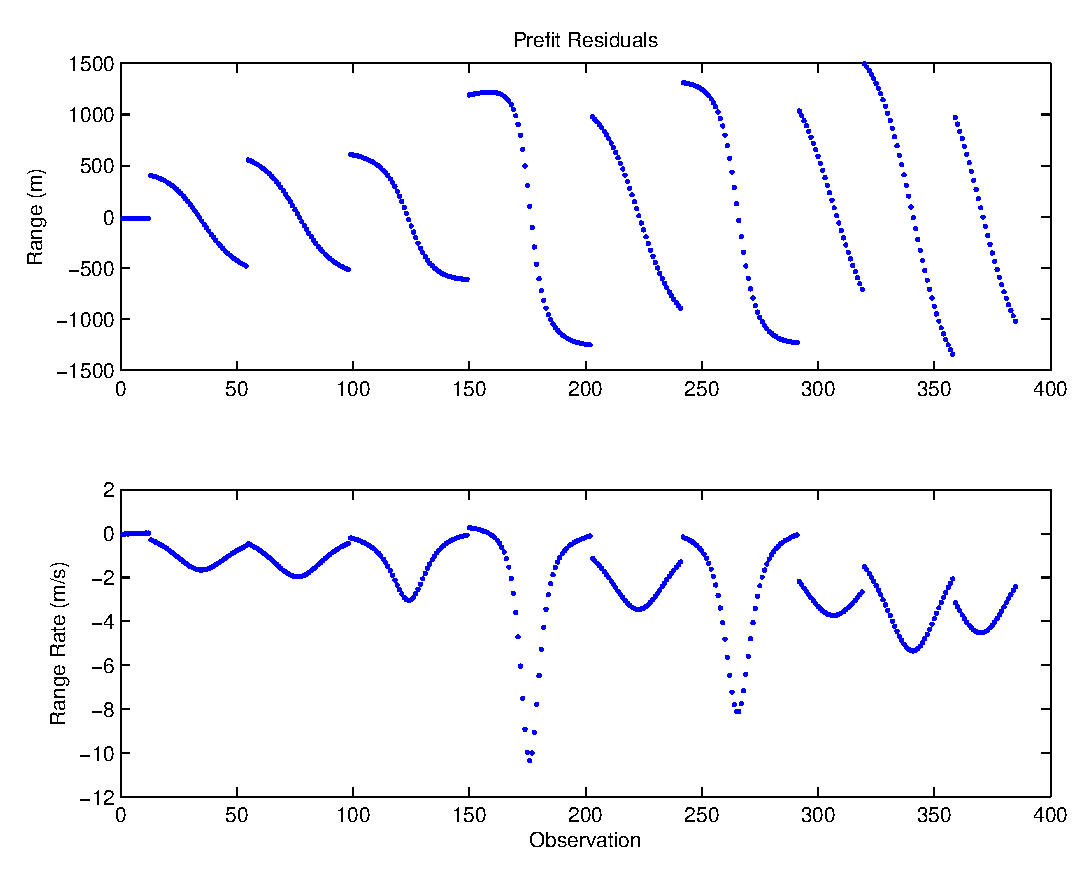
\includegraphics[width = 10cm]{Batch_Prefit.eps}
		\caption{Prefit residuals for range and range rate. }
		\label{fig:Prefit}
	\end{figure}	

	The estimated initial state (Table \ref{t:InitStates}) for both algorithms largely agrees with the \textit{a priori} state, save for the drag coefficient (Z$_{\text{site1}}$'s percent difference is an artifact due values close to 0). Table \ref{t:FinalStates} shows that the estimated final states for both aglorithms, as well as the percent difference between the both CKF $P$ formulations and the batch algorithm.
	\begin{table}[H]% no placement specified: defaults to here, top, bottom, page
		\begin{center}
			\caption{Initial state estimates.}
			\label{t:InitStates}
			\begin{tabular}{c|c|c|c|c}
\hline Element & Batch & CKF & \%-Diff & Units \\ \hline
$x$ &  757.7003e+003  & 757.7063e+003  & 789.9839e-006 & m\\
$y$  &   5.2226e+006  &   5.2226e+006 & 68.7216e-006 & m\\
$z$    & 4.8515e+006   &  4.8515e+006   & 34.3716e-006 & m\\
$\dot{x}$    & 2.2133e+003   &  2.2132e+003   &      1.0155e-003 & m/s\\
$\dot{y}$   &  4.6784e+003   &  4.6783e+003  & 947.1405e-006  & m/s\\
$\dot{z}$   & -5.3713e+003  &  -5.3713e+003  & 164.5647e-006 & m/s\\
$\mu$ &   398.6003e+012  & 398.6004e+012 & 34.5500e-006 & m\textsuperscript{3}/s\textsuperscript{2} \\
$J_2$ &     1.0801e-003   &  1.0826e-003 &   235.1557e-003  & --\\
$C_D$ &     2.7080e+000  &   2.0000e+000 & 26.1444e+000  & --\\
$X_{site1}$ &    -5.1275e+006 &   -5.1275e+006   &  90.8163e-015 & m\\
$Y_{site1}$ &    -3.7942e+006 &   -3.7942e+006  &  110.4580e-015 & m\\
$Z_{site1}$ &     1.4680e-009   &  0.0000e+000  &    100.0000e+000 & m\\
$X_{site2}$ &     3.8609e+006  &   3.8609e+006  & 888.7788e-006 & m\\
$Y_{site2}$ &     3.2385e+006  &   3.2385e+006  &   1.1111e-003 & m\\
$Z_{site2}$ &     3.8981e+006  &   3.8981e+006&  559.1565e-006 & m\\
$X_{site3}$ &   549.4842e+003 &   549.5050e+003 &  3.7872e-003 & m\\
$Y_{site3}$ &    -1.3809e+006 &   -1.3809e+006 & 609.0338e-006 & m\\
$Z_{site3}$ &     6.1822e+006  &   6.1822e+006 & 168.8545e-006  & m\\				
			\end{tabular}
		\end{center}
	\end{table}  	
	\begin{table}[H]% no placement specified: defaults to here, top, bottom, page
		\begin{center}
			\caption{Final state estimates.}
			\label{t:FinalStates}
			\begin{tabular}{c|c|c|c|c|c|c}
\hline &  &  & CKF-Batch &  & Joseph-Batch & \\
Element & Batch & CKF & \%-Diff & CKF-Joseph & \%-Diff & Units\\ \hline
$x$         & 1.1286e+006   & 1.1286e+006    &     24.7049e-006 & 1.1286e+006    &     35.7141e-006 & m\\
$y$         & 5.9901e+006   & 5.9901e+006    &      1.2996e-006 & 5.9901e+006    &      1.5631e-006 & m\\
$z$         & 3.7754e+006   & 3.7754e+006    &     17.5277e-006 & 3.7754e+006    &     15.7053e-006 & m\\
$\dot{x}$   & 2.0092e+003   & 2.0092e+003    &     41.6678e-006 & 2.0092e+003    &     28.9850e-006 & m/s\\
$\dot{y}$   & 3.5630e+003   & 3.5630e+003    &     11.4093e-006 & 3.5630e+003    &     11.0051e-006 & m/s\\
$\dot{z}$   & -6.2376e+003  & -6.2376e+003   &      5.8644e-006 & -6.2376e+003   &      7.7204e-006 & m/s\\
$\mu$       & 398.6003e+012 & 398.6004e+012  &     21.5797e-006 & 398.6004e+012  &     22.1143e-006 & m\textsuperscript{3}/s\textsuperscript{2}\\
$J_2$       & 1.0807e-003   & 1.0820e-003    &    116.2359e-003 & 1.0820e-003    &    116.5768e-003 & --\\
$C_D$       & 2.5212e+000   & 2.1555e+000    &     14.5059e+000 & 2.1446e+000    &     14.9369e+000 & --\\
$X_{site1}$ & -5.1275e+006  & -5.1275e+006   &     35.7634e-012 & -5.1275e+006   &     33.7655e-012 & m\\
$Y_{site1}$ & -3.7942e+006  & -3.7942e+006   &     35.7638e-012 & -3.7942e+006   &     33.7756e-012 & m\\
$Z_{site1}$ & 676.0602e-012 & -249.3974e-009 &     36.9898e+003 & -276.4921e-009 &     40.9976e+003 & m\\
$X_{site2}$ & 3.8609e+006   & 3.8609e+006    &    518.7581e-006 & 3.8609e+006    &    519.4818e-006 & m\\
$Y_{site2}$ & 3.2385e+006   & 3.2385e+006    &    618.9084e-006 & 3.2385e+006    &    623.4447e-006 & m\\
$Z_{site2}$ & 3.8981e+006   & 3.8981e+006    &    306.5495e-006 & 3.8981e+006    &    305.3395e-006 & m\\
$X_{site3}$ & 549.4892e+003 & 549.4992e+003  &      1.8291e-003 & 549.4993e+003  &      1.8465e-003 & m\\
$Y_{site3}$ & -1.3809e+006  & -1.3809e+006   &    296.6497e-006 & -1.3809e+006   &    313.1818e-006 & m\\
$Z_{site3}$ & 6.1822e+006   & 6.1822e+006    &     96.6940e-006 & 6.1822e+006    &     96.9202e-006 & m\\			
			\end{tabular}
		\end{center}
	\end{table}  

	The postfit residuals can be seen in Figures \ref{fig:BatchPostfit} and \ref{fig:CKFPostfit}:

	\begin{figure}[H]
		\centering
		\includegraphics[width = 10cm]{Batch_PostFit.eps}
		\caption{Postfit residuals for range, range rate using batch algorithm. Shown with 3$\sigma$ measurement envelopes. }
		\label{fig:BatchPostfit}
	\end{figure}	
	\begin{figure}[H]
		\centering
		\subfigure[Conventional covariance formulation]{
			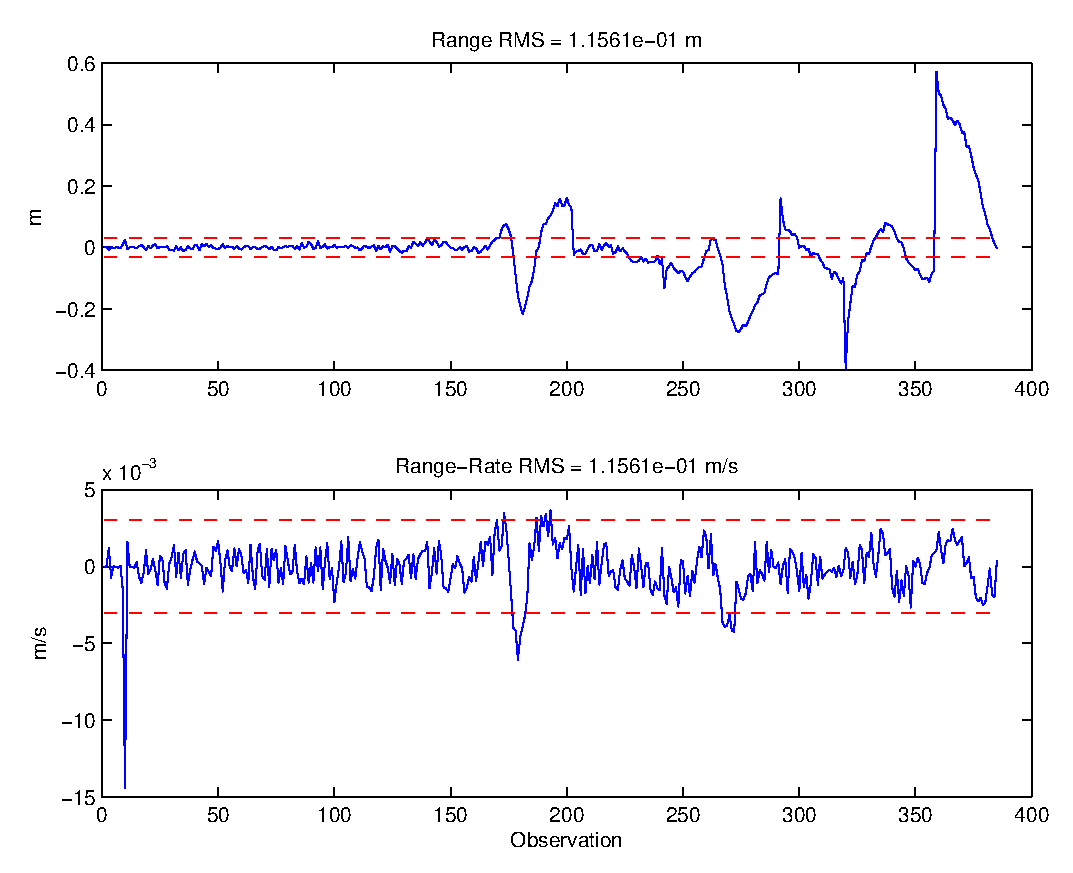
\includegraphics[width = 7cm]{CKF_PostFit.eps}
		}
		\subfigure[Joseph covariance formulation]{
			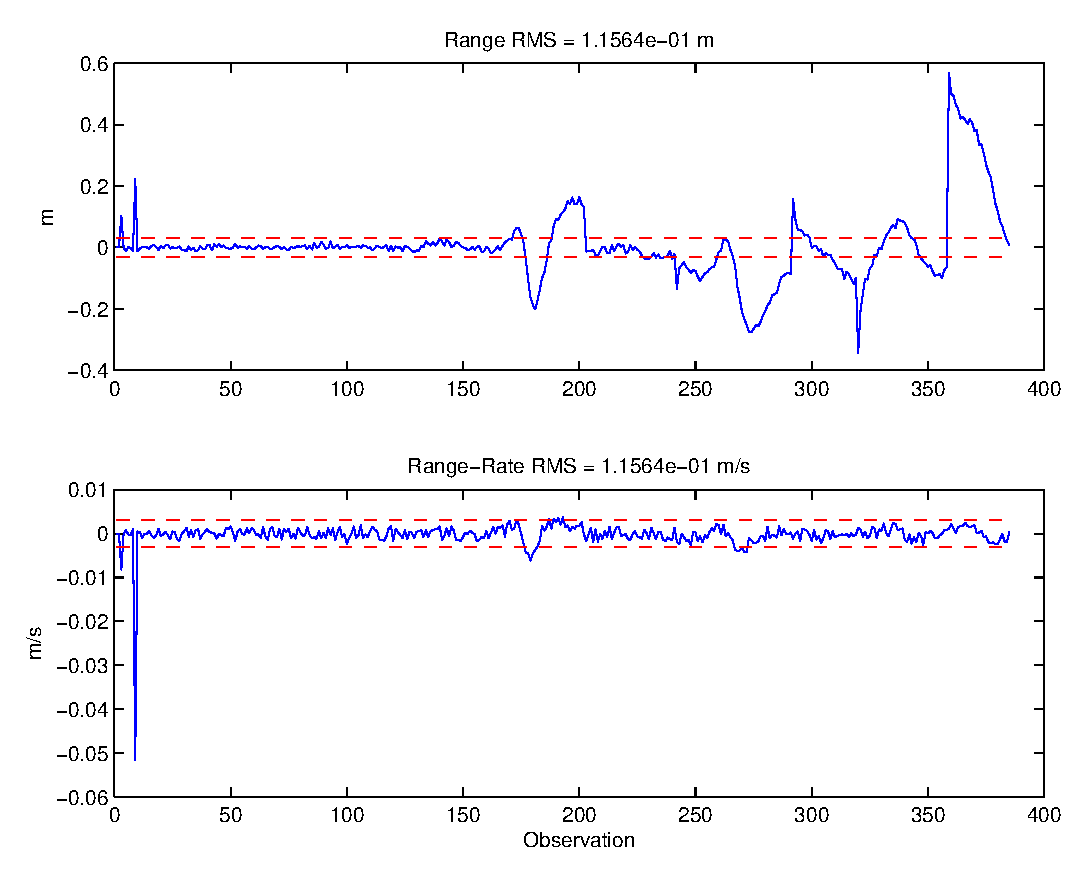
\includegraphics[width = 7cm]{CKF_Joseph_PostFit.eps}
		}
		\caption{Postfit residuals for range, range rate using batch algorithm. Shown with 3$\sigma$ measurement envelopes. }
		\label{fig:CKFPostfit}
	\end{figure}	

	The traces of the covariance matrix is shown in Figure \ref{fig:CKF_Cov} for both the conventional and Joseph formulations of $P$:

	\begin{figure}[H]
		\centering
		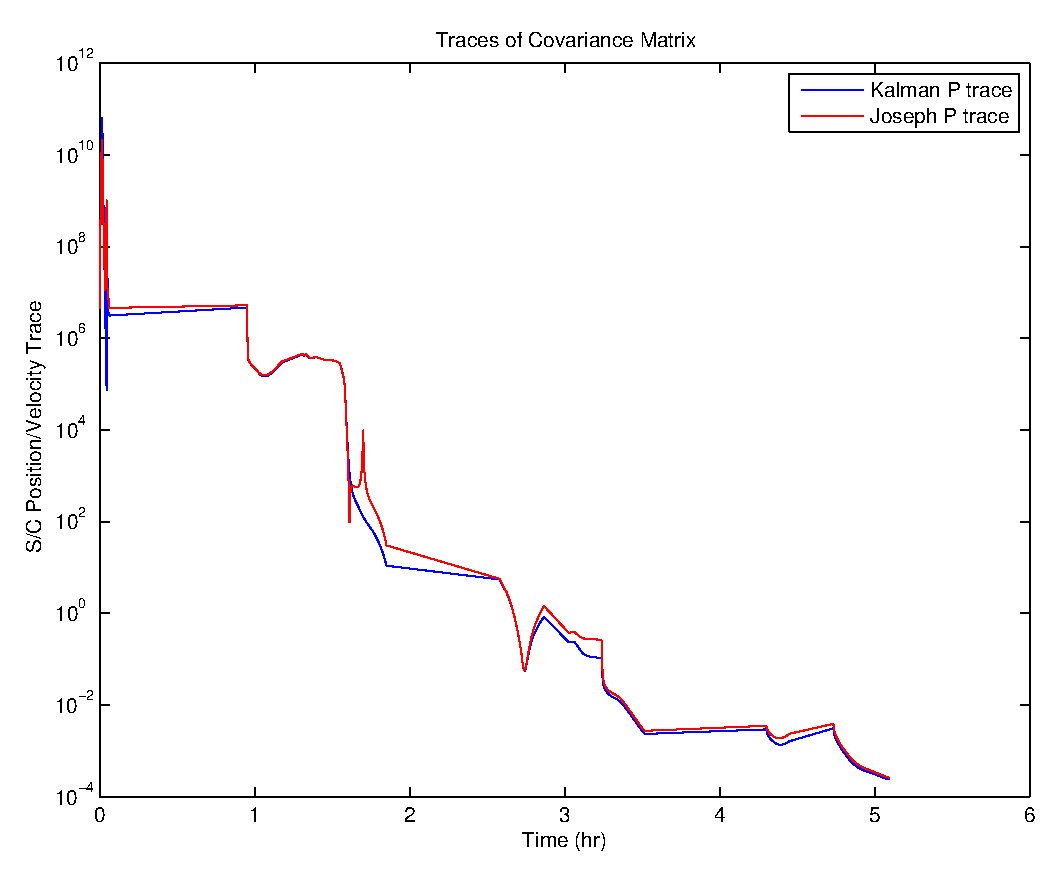
\includegraphics[width = 10cm]{CKF_Cov.eps}
		\caption{Covariance trace for position and velocity components, CKF. }
		\label{fig:CKF_Cov}
	\end{figure}	

	Finally, the error ellipsoids for both algorithms can be seen in Figure \ref{fig:ErrorEllipsoids}.

	\begin{figure}[H]
		\centering
		\subfigure[Batch Algorithm]{
			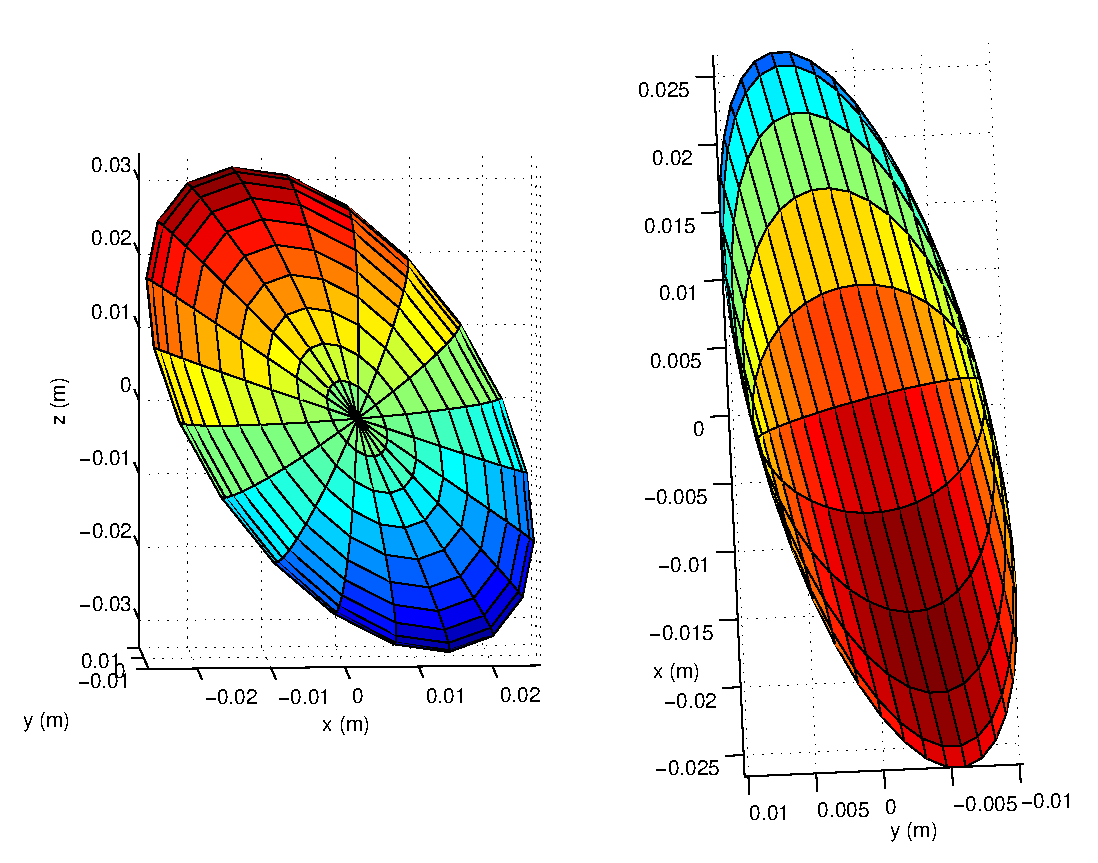
\includegraphics[width = 7cm]{Batch_Ellipsoid_Final.eps}
		}
		\subfigure[CKF Algorithm]{
			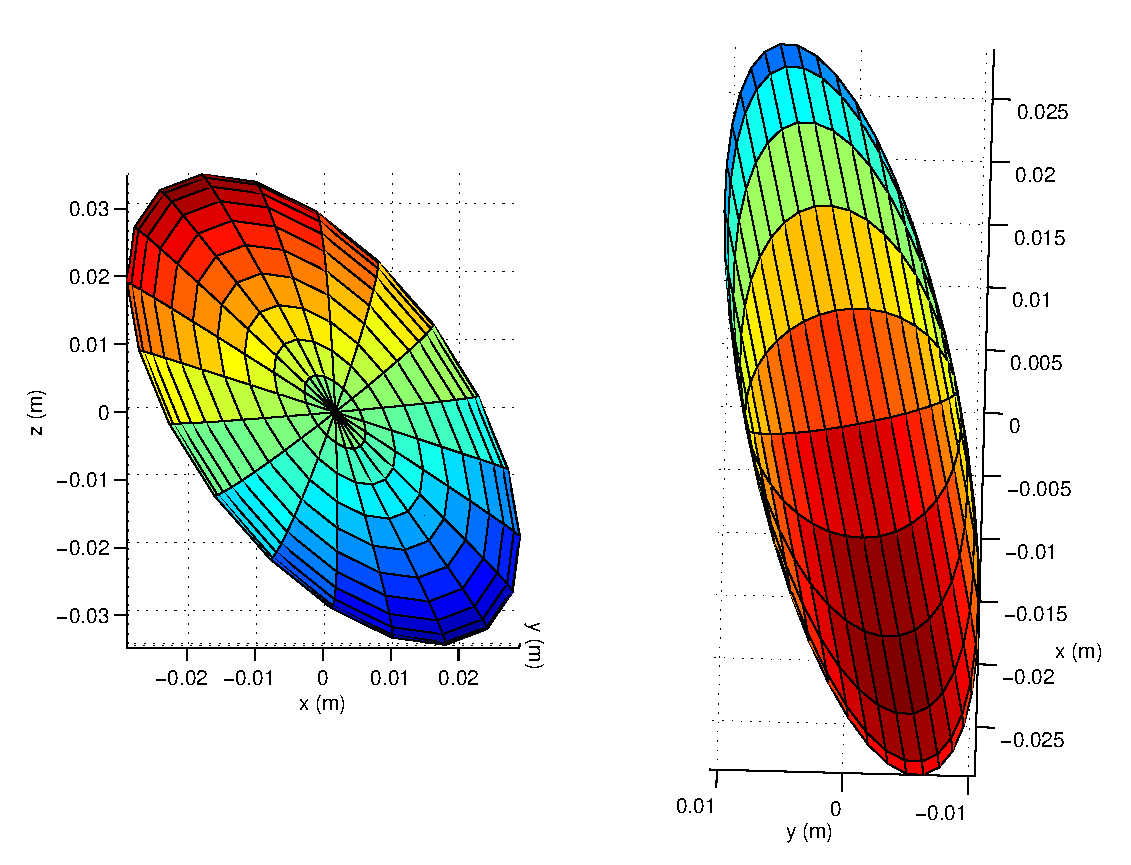
\includegraphics[width = 7cm]{CKF_Ellipsoid_Final.eps}
		}
		\caption{3$\sigma$ error ellipsoids. }
		\label{fig:ErrorEllipsoids}
	\end{figure}	

	\section{Discussion: Batch vs. CKF}
	
	The postfit residuals indicate whether or not an algorithm was within the measurement 3$\sigma$ error bars.  The batch algorithm performed well in this regard; all residuals were within the error envelope within the second pass. Neither implementation of the CKF stayed within the 3$\sigma$ envelopes in one pass, although both had better range RMS values than the first pass of the batch algorithm. Batch had a lower RMS for range rate in the first pass compared to both CKF formulations, mostly due to an outlier residual on the 9th observation.  At this point, the CKF was still susceptible to noise in the measurements because it has had few prior measurements process beforehand.  The Joseph formulation of the CKF encountered similar issues in the range residuals, although they were quite small compared to the divergence of the residuals after $\sim$160 observations.  The Joseph formulation kept the covariance matrix symmetric, which explains the difference.  Symmetry can be lost in the conventional formulation of the covariance when a large \textit{a priori} covariance is processed with accurate measurements due to finite machine precision\cite{Born}.
	
	\vspace{5 mm}

	The impact of the Joseph formulation of the CKF covariance can be seen in Figure \ref{fig:CKF_Cov}. The Joseph formulation stayed slightly higher throughout, as $P$ kept its symmetry.  The variance of the CKF collapses as measurements were processed, making the filter consider measurements less as time progresses. The batch algorithm did not have this issue because it processed \textit{a priori} information like it would a measurement. Adding process noise, which would keep the covariance from collapsing, would help the CKF keep considering new measurements as time progresses.  
	
	\vspace{5 mm}

	Additionally, the batch algorithm was less susceptible to errors induced by covariance matrices, because a poorly conditioned information matrix (which required one inversion of the \textit{a priori} covariance matrix) was only inverted once to get the covariance matrix.  For this implementation of the batch algorithm, Cholesky decomposition was performed to reduce the error resulting in performing an inverse of a poorly conditioned matrix. The CKF, on the other hand, multiplied the \textit{a priori} three times per observation epoch, as well as inverted one of the products.  Error in the covariance was thus introduced and propagated at every observation epoch, even with the Joseph formulation (which became non-positive definite at times). Thus, the batch algorithm had a more accurate solution for $P$ due to computer precision. A square-root method for the CKF would reduce the condition of the matrix containing the uncertainty information by a factor of 2. Such a method would result in a more accurate covariance matrix that would stay symmetric and positive definite.
	
	\vspace{5 mm}

	The final error ellipsoids for the spacecraft position between the two algorithms were close in size and direction.  The CKF had more uncertainty in the x and z directions. As discussed previously, the batch result was the more reliable of the two.
	
	\section{Processing of Only One Measurement Type}
	
	The effects of measurement type (range or range rate) were analyzed.  The batch algorithm was run with the same conditions and \textit{a priori} knowledge, but processed once with only range measurements, and once with only range rate measurements.  The relative differences of the estimated initial and final states with the dual-measurement batch solution are shown in Table \ref{t:SingleMeasDiff}.  Postfit residuals for both runs are shown in Figure \ref{fig:Postfit_Single_meas}, and the 3$\sigma$ position error are shown in Figure \ref{fig:ErrorEllipsoids_Single_meas}.

	\begin{table}[H]% no placement specified: defaults to here, top, bottom, page
		\begin{center}
			\caption{Single-measurement type percent differences with both measurement types.}
			\label{t:SingleMeasDiff}
			\begin{tabular}{c|c|c|c|c}
\hline & Init. State & Init. State & Final State & Final State \\
 & Range Only & Range-Rate Only & Range Only & Range-Rate Only\\ 
Element & \%-Diff & \%-Diff & \%-Diff & \%-Diff\\ \hline
$x$         &     13.1303e-009  &   9.6290e-006 &   14.8102e-006 &   14.8102e-006 \\
$y$         &    882.1571e-012  &  13.6724e-006 &    9.3189e-006 &    9.3189e-006 \\
$z$         &      7.5071e-009  &   4.3868e-006 &    1.0470e-006 &    1.0470e-006 \\
$\dot{x}$   &    442.1213e-012  &   3.6962e-006 &   10.4436e-006 &   10.4436e-006 \\
$\dot{y}$   &    877.2484e-012  &   3.7360e-006 &    2.6213e-006 &    2.6213e-006 \\
$\dot{z}$   &      5.4108e-009  &  10.8486e-006 &    6.2054e-006 &    6.2054e-006 \\
$\mu$       &      1.7415e-009  & 152.0529e-006 &  135.7060e-006 &  135.7060e-006 \\
$J_2$       &      1.0009e-006  &  11.8443e-003 &   11.0662e-003 &   11.0662e-003 \\
$C_D$       &     19.2734e-003  &  15.4194e+000 &   15.7782e+000 &   15.7782e+000 \\
$X_{site1}$ &     18.1633e-015  &  90.8163e-015 &   90.8163e-015 &   90.8163e-015 \\
$Y_{site1}$ &     24.5462e-015  & 110.4580e-015 &   98.1848e-015 &   98.1848e-015 \\
$Z_{site1}$ &      9.4487e+000  & 109.5868e+000 &  121.9467e+000 &  121.9467e+000 \\
$X_{site2}$ &     42.9717e-009  &  35.1569e-006 &   28.0806e-006 &   28.0806e-006 \\
$Y_{site2}$ &     24.9975e-009  &  50.5199e-006 &   38.5169e-006 &   38.5169e-006 \\
$Z_{site2}$ &      7.2785e-009  &  31.4754e-006 &   37.1453e-006 &   37.1453e-006 \\
$X_{site3}$ &     78.5123e-009  &  26.2115e-006 &   67.0482e-006 &   67.0482e-006 \\
$Y_{site3}$ &     48.9074e-009  & 187.7865e-006 &  155.8026e-006 &  155.8026e-006 \\
$Z_{site3}$ &     12.6907e-009  &  34.7815e-006 &   28.4767e-006 &   28.4767e-006 \
			\end{tabular}
		\end{center}
	\end{table}  

	\begin{figure}[H]
		\centering
		\subfigure[Range only]{
			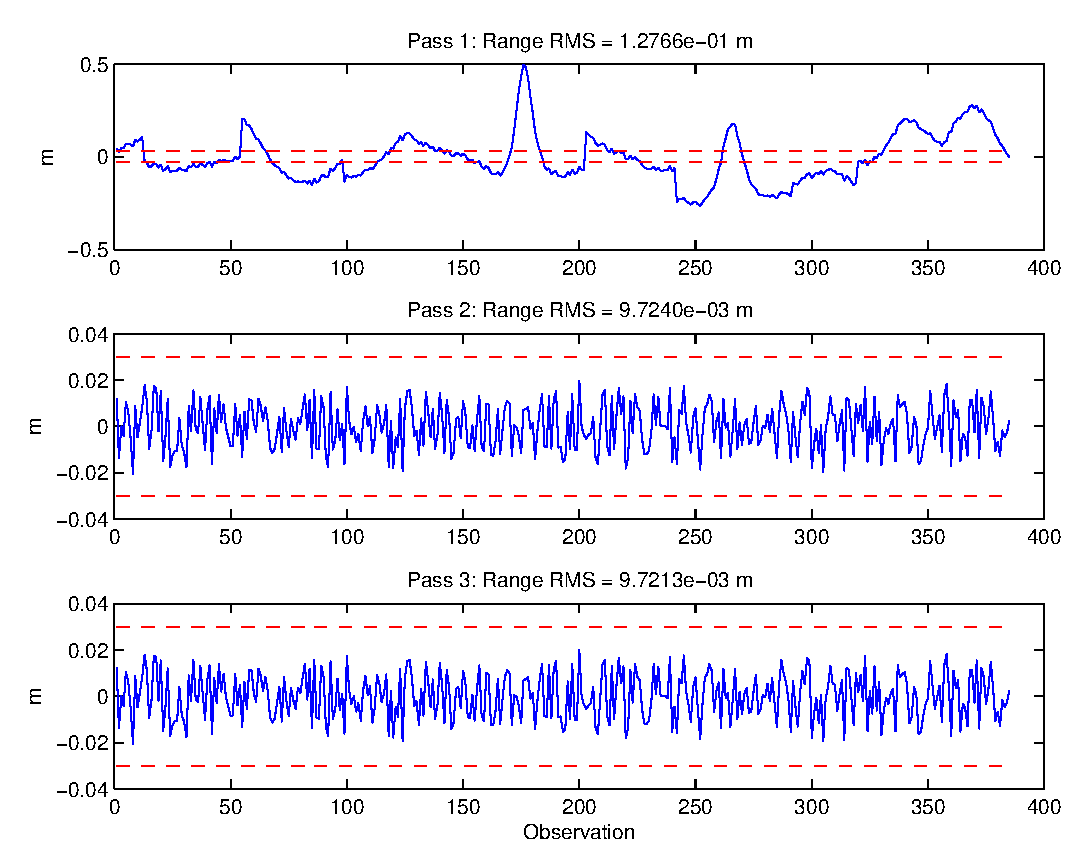
\includegraphics[width = 7cm]{R_only_Postfit.eps}
		}
		\subfigure[Range rate only]{
			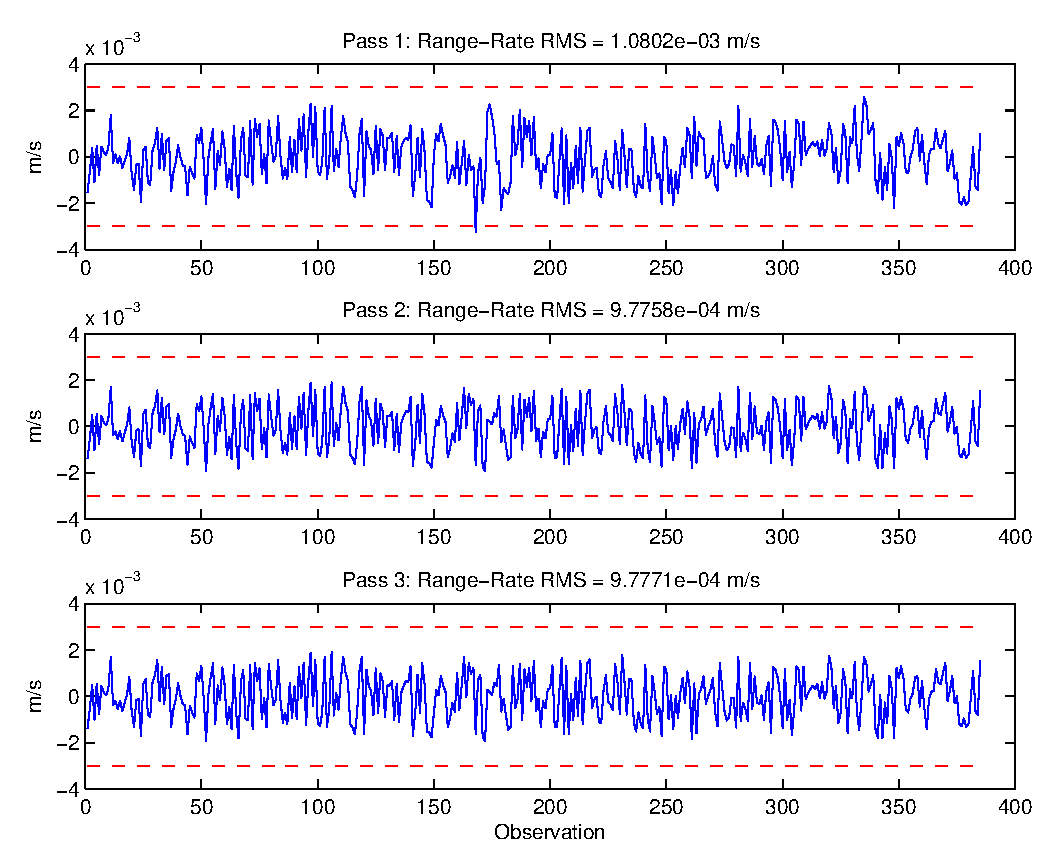
\includegraphics[width = 7cm]{RR_only_Postfit.eps}
		}
		\caption{Postfit residuals from processing one measurement type, batch algorithm. }
		\label{fig:Postfit_Single_meas}
	\end{figure}	

	\begin{figure}[H]
		\centering
		\subfigure[Range only]{
			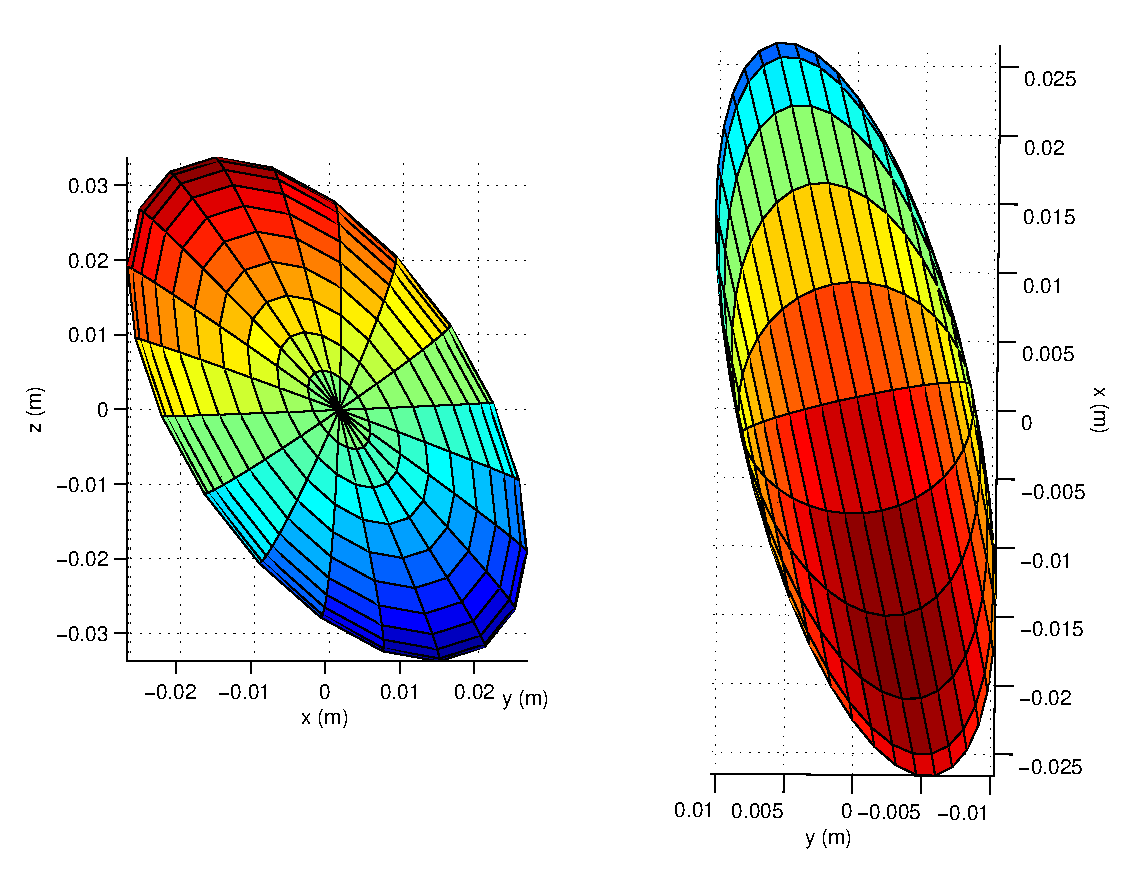
\includegraphics[width = 7cm]{R_only_Ell.eps}
		}
		\subfigure[Range rate only]{
			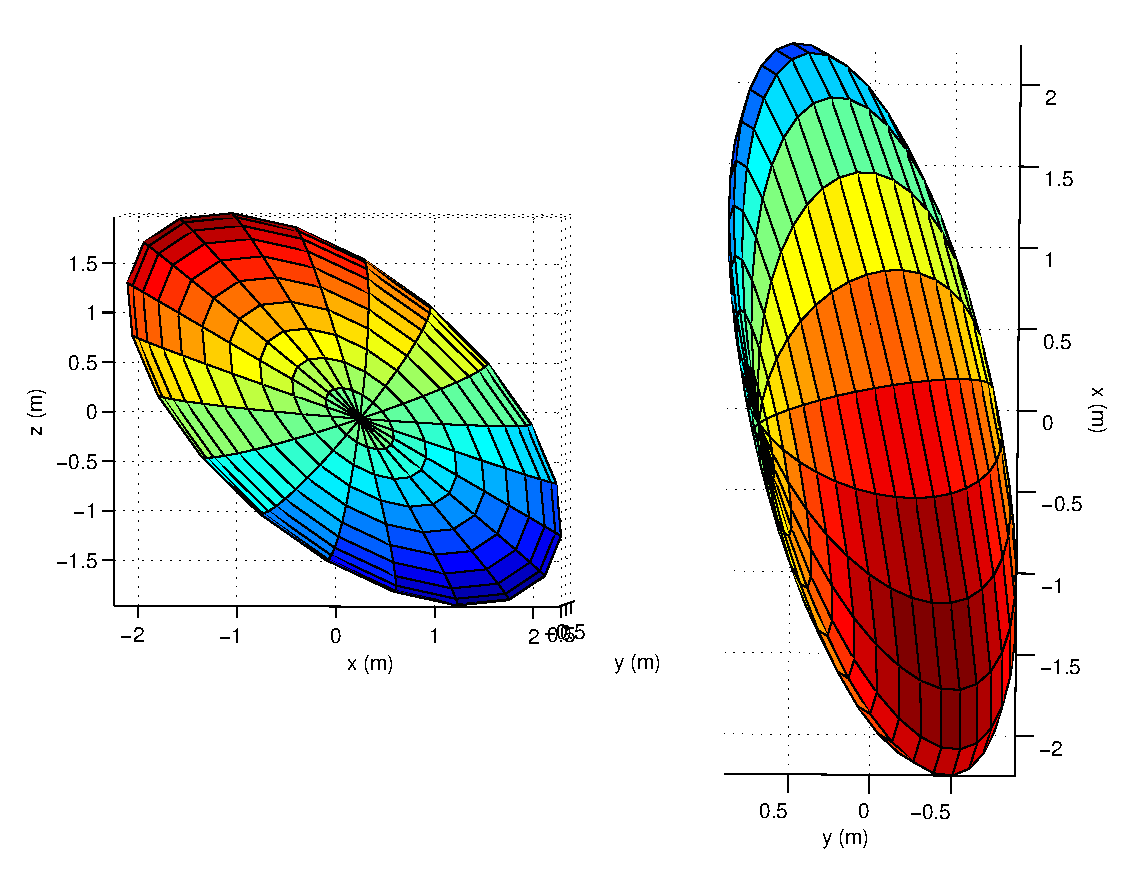
\includegraphics[width = 7cm]{RR_only_Ell.eps}
		}
		\caption{3$\sigma$ error ellipsoids using only one measurement type, batch algorithm. }
		\label{fig:ErrorEllipsoids_Single_meas}
	\end{figure}	

	The drag coefficient showed the most error with the previous solution (Z$_{\text{site1}}$'s error was on the scale of nanometers). This was expected since the previous solution was so far off from \textit{a priori} knowledge anyway, as neither measurement type was very sensitive to C$_{\text{D}}$ in the first place (compared to other state elements).
	
	\vspace{5 mm}

	The postfit residuals were within the error bars of the measurements in the final pass of the algorithm.  The range RMS values were very close to that of the batch process with both measurement types.  The range-rate RMS, however, was slightly smaller.  This was due to the smaller variance of the range-rate measurement, which made the postfit resuduals less tightly bound around zero in the presence of larger variance data.
	
	\vspace{5 mm}

	The positions error ellipsoids demonstrated the effect that measurement sensitivity can have, despite the accuracy of the measurements.  The range-only ellipsoid was quite similar to the dual-measurement case. However, the range-rate-only ellipsoid was orders of magnitude larger, despite the smaller variance in the measurement. Recall Equation \ref{eq:BLS}. The measurement sensitivity matrix was the culprit here, with the accumulated values for each observation epoch being an order of magnitude smaller for range rate than for range.  So despite the accurate data, the range-rate-only solution had more variance simply because the measurements were less sensitive to changes in the state elements.  Table \ref{t:Meas_sensitivity_sums} demonstrates the overall measurement sensitivity to the state elements by summing all of the elements of $H$ for all measurement epochs.  

	\begin{table}[H]% no placement specified: defaults to here, top, bottom, page
		\begin{center}
			\caption{Measurement senisitivity sums.}
			\label{t:Meas_sensitivity_sums}
			\begin{tabular}{|c|c|}
\hline
$\Sigma H_{range}$         &     -264.0064e+006   \\ \hline
$\Sigma H_{range rate}$ &     -45.5771e+006  \\ \hline
			\end{tabular}
		\end{center}
	\end{table}  
	
	\section{Ground Station Knowledge}
	
	The effects of ground station position confidence was tested by fixing each of the ground stations individually by reducing their position variances to $10^{-10}$.  The case of all ground stations having a large position variance was also examined.  The estimated state relative differences are shown in Table \ref{t:GSFixed} in the Appendix; the postfit residuals and error ellipsoids are displayed in Figures \ref{fig:Postfit_GS} and \ref{fig:ErrorEllipsoids_GS}.
		
	\begin{figure}[H]
		\centering
		\subfigure[Turkey site fixed]{
			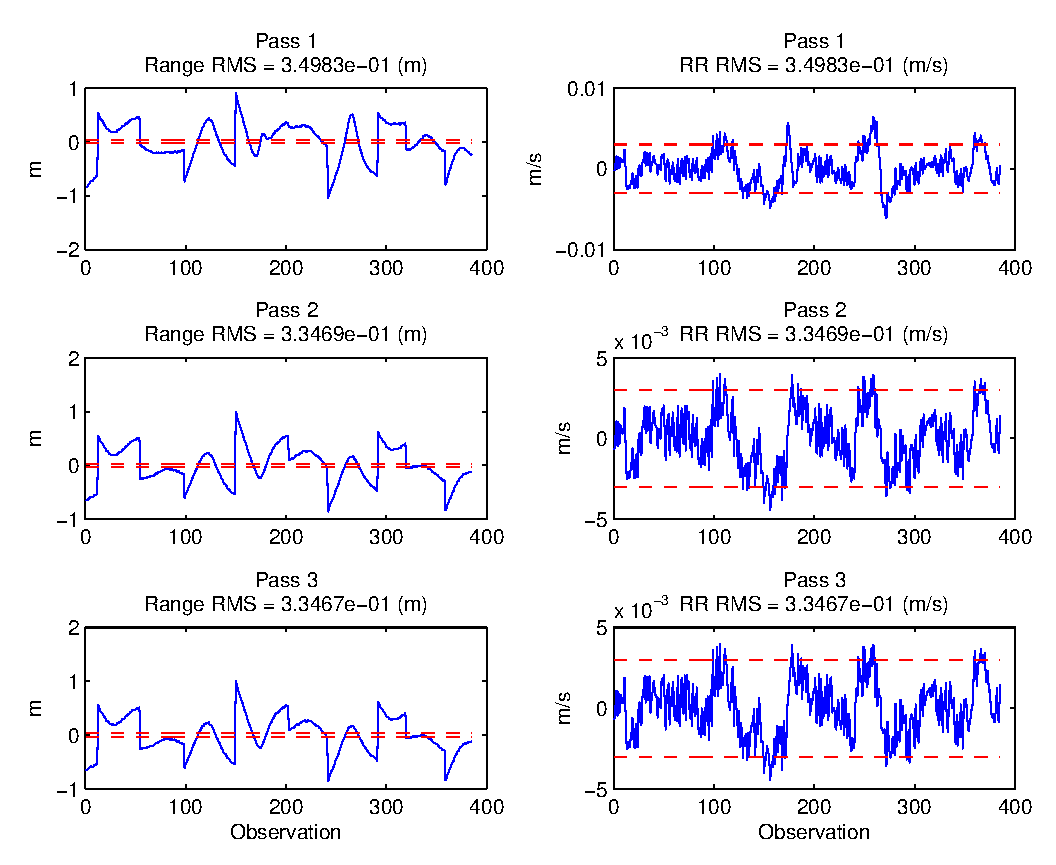
\includegraphics[width = 7cm]{GS_Turk_PFR.eps}
		}
		\subfigure[Greenland site fixed]{
			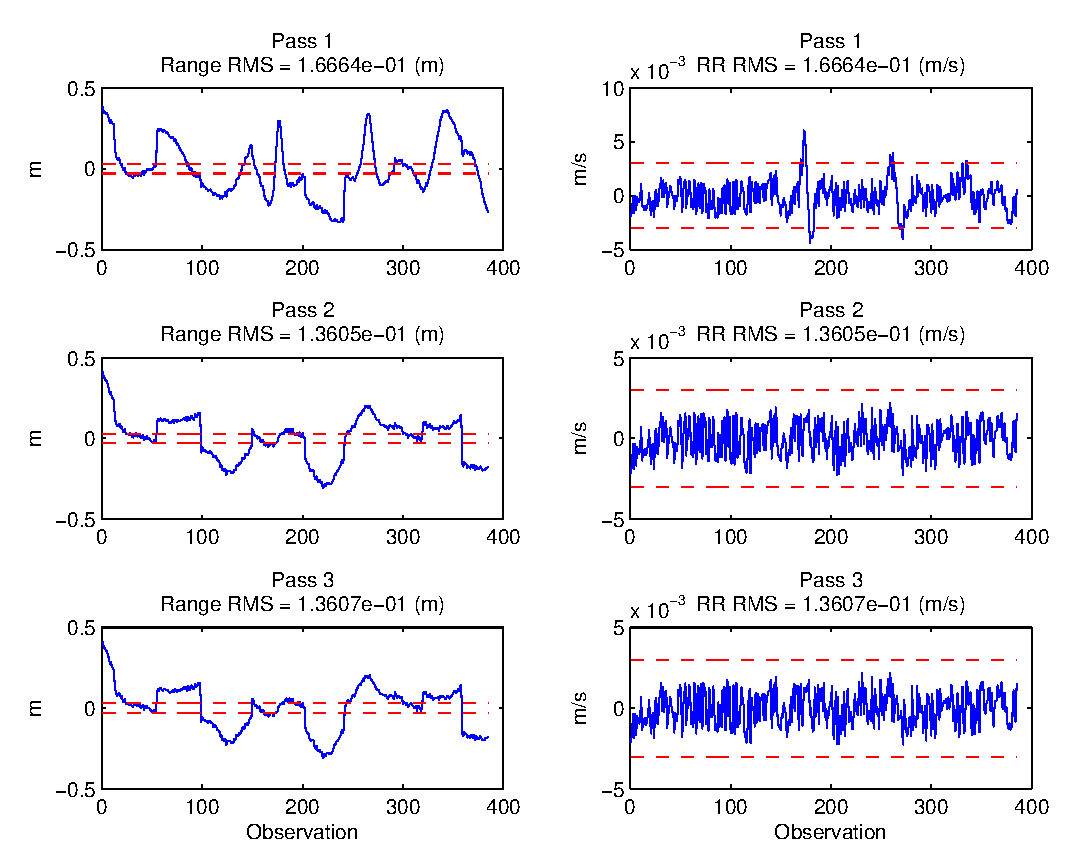
\includegraphics[width = 7cm]{GS_Gnld_PFR.eps}
		}
		\subfigure[No sites fixed]{
			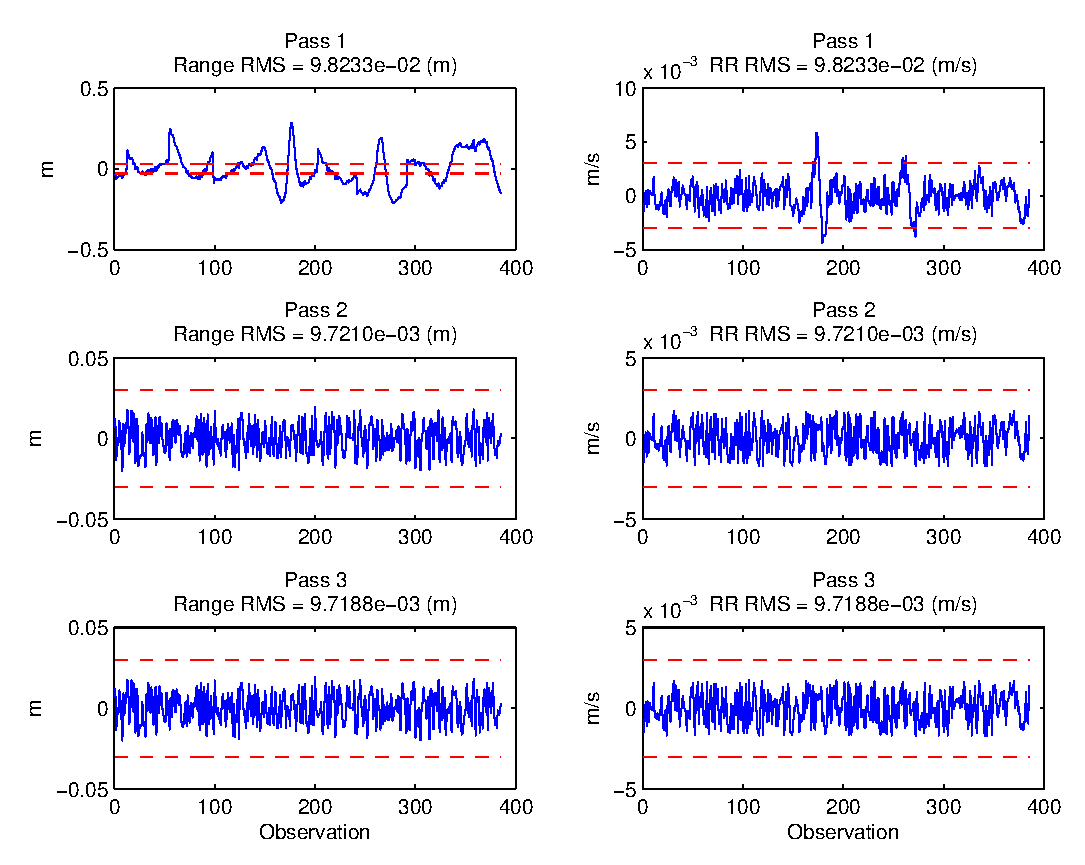
\includegraphics[width = 7cm]{GS_none_PFR.eps}
		}
		\caption{Postfit residuals from fixing various ground sites, batch algorithm. }
		\label{fig:Postfit_GS}
	\end{figure}	

	\begin{figure}[H]
		\centering
		\subfigure[Turkey site fixed]{
			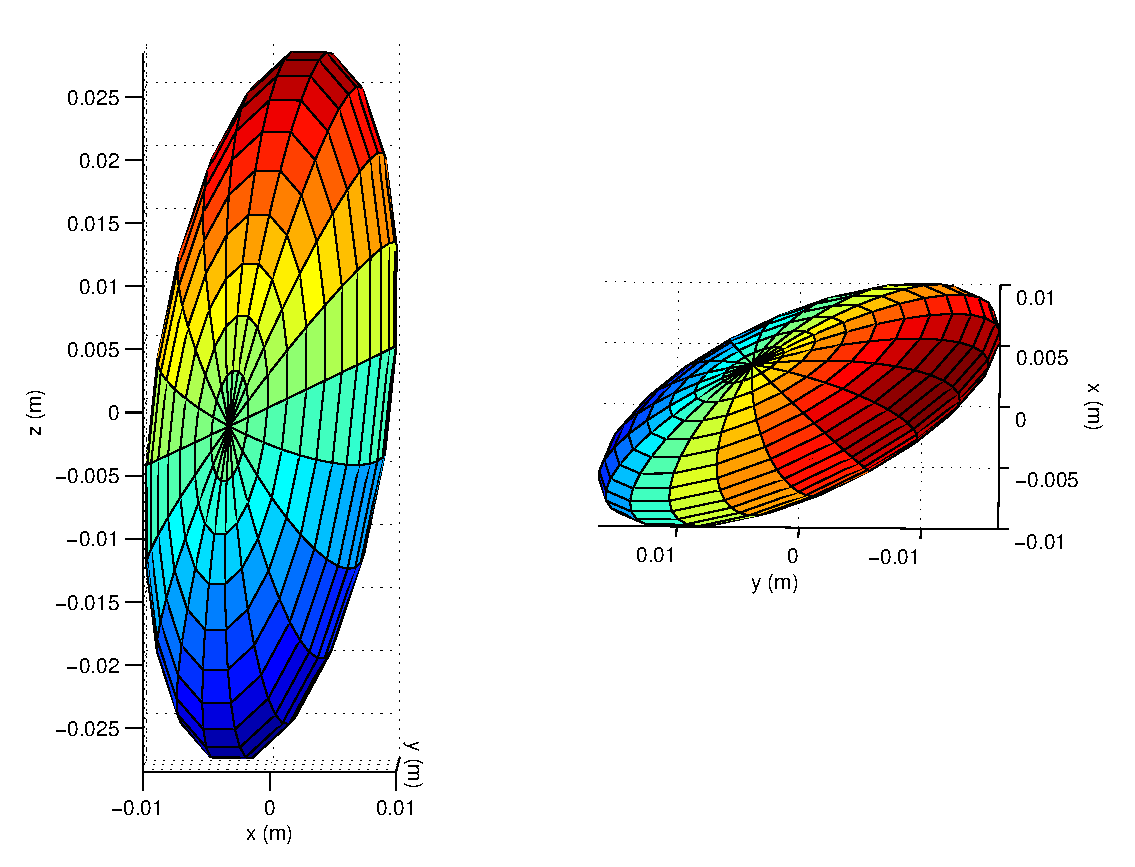
\includegraphics[width = 7cm]{GS_Turk_Ell.eps}
		}
		\subfigure[Greenland site fixed]{
			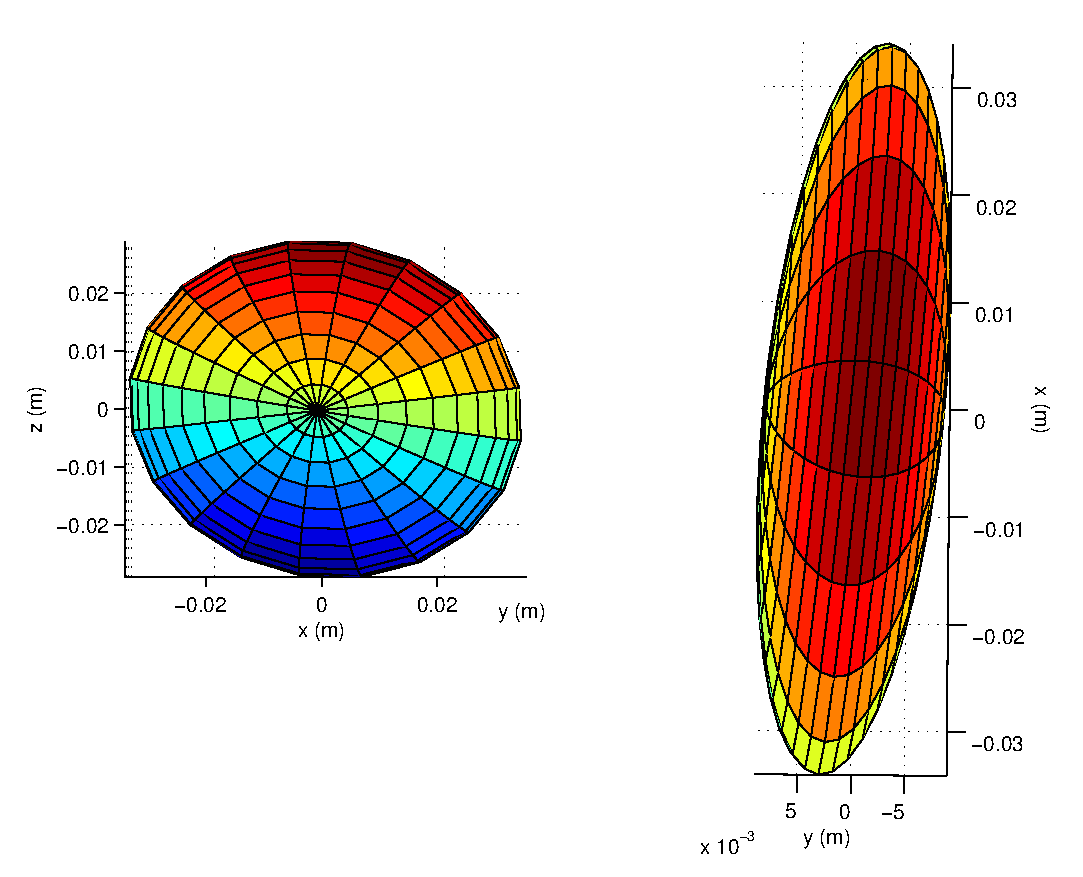
\includegraphics[width = 7cm]{GS_Gnld_Ell.eps}
		}
		\subfigure[No sites fixed]{
			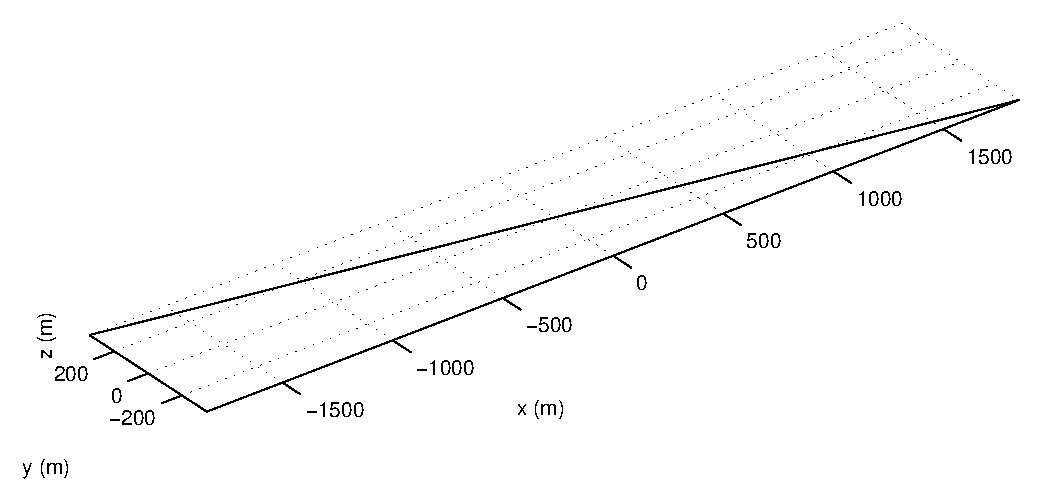
\includegraphics[width = 7cm]{GS_none_Ell.eps}
		}
		\caption{3$\sigma$ error ellipsoids from fixing various ground sites, batch algorithm. }
		\label{fig:ErrorEllipsoids_GS}
	\end{figure}	

	For the Turkey and Greenland sites being fixed, the postfit residuals for range weren't within the measurement error envelope. The position error ellipsoids were similar in magnitude to that of the Pacific-fixed site.  In contrast, fixing none of the sites resulted in residuals within measurement error, but a position error ellipsoid with a semi-major axis of almost 4 km!  An analysis of the ground track during the observations offered insight to these findings.  Figure \ref{fig:GroundTrack} shows where each ground site observed the spacecraft.

	\begin{figure}[H]
		\centering
		\includegraphics[width = 10cm]{CoveragePlot.jpg}
		\caption{Ground track of spacecraft during observations. Courtesy CCAR. }
		\label{fig:GroundTrack}
	\end{figure}	

	The Pacific site was near-directly under one of the one of the passes, and it observed the satellite at its maximum rate of latitude change. This gave the site the best geometry for range measurements on that pass.  Additional study into the effect of measurement site and satellite geometry that included azimuth and elevation measurements would help test this hypothesis. 

	\section{Potter Square Root Formulation for the CKF}

	The Potter formulation of the CKF is one of a few square-root methods used to avoid saturation due to numerical error in the measurement update of $P$. Such methods define $P=WW^T$ so that it can work on the square root of the covariance matrix, W. The result is that $W$ has half the log of the conditioning number of $P$, and the generation of $P$ from $W$ leads to a symmetric, positive definite matrix. From the measurement update in equation \ref{eqn:MeasUpdate}, the update can become

	\begin{equation}
	WW^T=\bar{W}[I-\tilde{F}\alpha\tilde{F}]W^T=\bar{W}\tilde{A}\tilde{A}^TW^T
	\end{equation}

	\noindent where

	\begin{equation}
	\tilde{F}=\bar{W}^TH^T,\alpha=(\tilde{F}^T\tilde{F}+R)^{-1}
	\end{equation}

	Potter found that by processing measurements independently during an observation epoch, $\tilde{A}$ could be found to be
	\begin{equation}
	\tilde{A}=[I-\gamma\alpha\tilde{F}\tilde{F}]
	\end{equation}

	\noindent due to $\alpha$ being scalar.  Using the quadratic formula, $\gamma$ is found to be 
	\begin{equation}
	\gamma=(1+\sqrt{R\alpha})^{-1}
	\end{equation}

	The Potter formulation of the CKF was implemented and processed the same data as the CKF.  The final state estimate's relative difference to the batch solution is found in Table \ref{t:Potter_results}.  The postfit residuals and covariance trace are shown in Figures \ref{fig:Potter_Postfit} and \ref{fig:Potter_Cov}, respectively

	\begin{figure}[H]
		\centering
		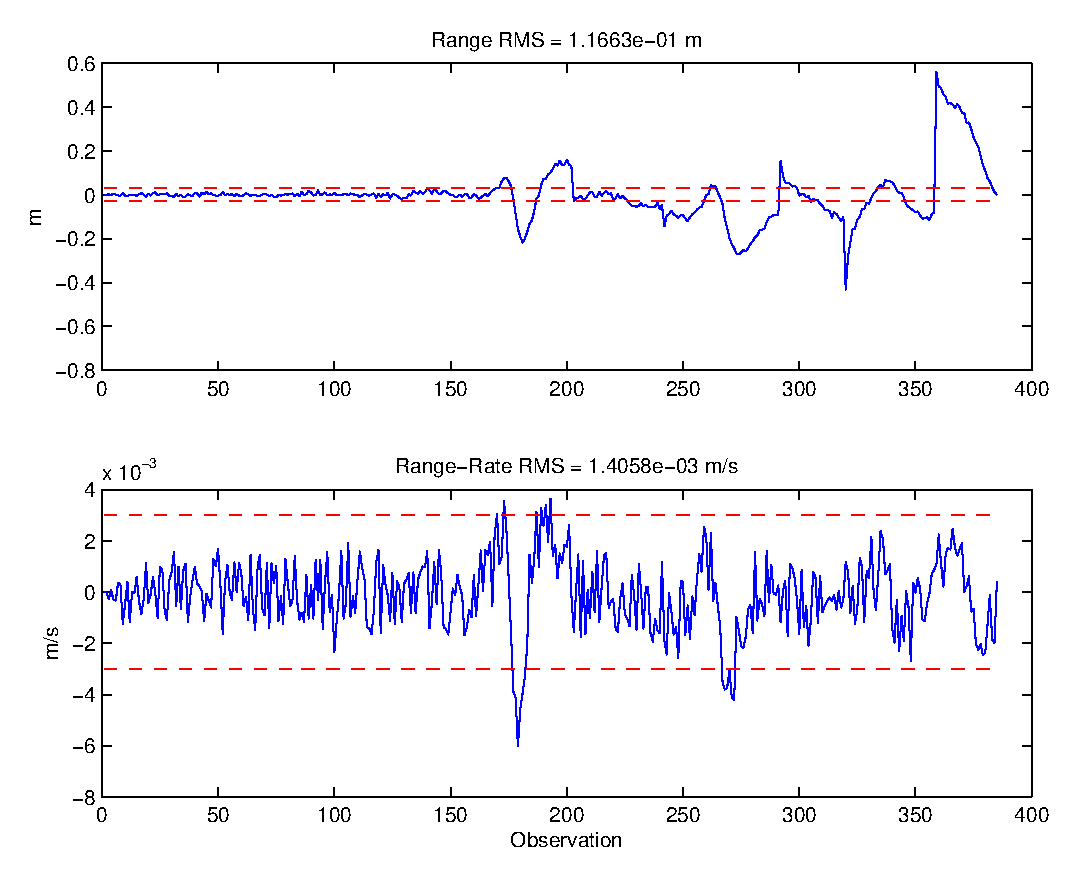
\includegraphics[width = 10cm]{Potter_Postfit.eps}
		\caption{CKF postfit residuals using Potter formulation }
		\label{fig:Potter_Postfit}
	\end{figure}	
	\begin{figure}[H]
		\centering
		\includegraphics[width = 10cm]{Potter_Cov.eps}
		\caption{Potter-formulated covariance vs. other CKF formulations. }
		\label{fig:Potter_Cov}
	\end{figure}	

	The postfit residuals stayed within the measurement accuracy envelope up to 160 observations, after which the filter diverges.  This result was notable because the conventional and Joseph formulations of $P$ led to large residuals in the first several observations. The estimated states and residuals weren't necessarily better than the previous CKF solutions, but the covariance was more accurate since it stayed symmetric and positive definite while suffering from less machine-precision error. This advantage did not stave off filter divergence, however; process noise and/or use of the extended Kalman filter should be used to rectify the issue.
	
	\vspace{5 mm}

	The effect of the calculation and use of $W$ instead of $P$ is seen in Figure \ref{fig:Potter_Cov}. Note that the covariance trace wasn't better because it was generally smaller than the others. The Potter trace was a better representation than the others due to how it is calculated.  There were observation epochs where the other algorithms diverged from the Potter covariance trace by an order of magnitude or more.  Such errors could lead the filter to diverge, if the covariance matrix was so small measurements were ignored.

	\section{Varying Data Noise and \textit{A Priori} Covariance Matrices}
	
	The data noise covariance $R$ was varied by increasing both measurement standard deviations by a factor of 10, decreasing them by a factor of ten, and decreasing only the range measurement standard deviation by a factor of ten.  The postfit residuals/RMS and error ellipsoids for the batch solution are shown in Figures \ref{fig:Postfit_DN} and \ref{fig:ErrorEll_DN}.

	\begin{figure}[H]
		\centering
		\subfigure[Increased both noise variance]{
			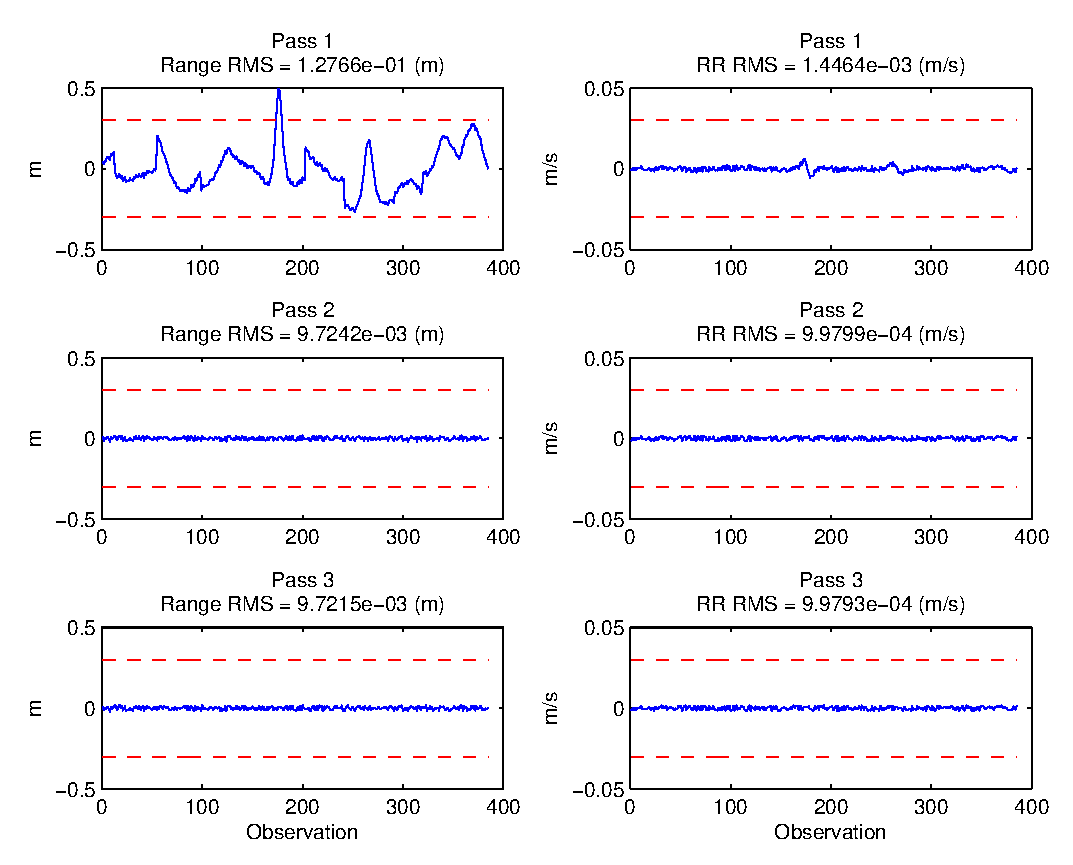
\includegraphics[width = 7cm]{DataNoise_inc_PFR.eps}
		}
		\subfigure[Decreased both noise variance]{
			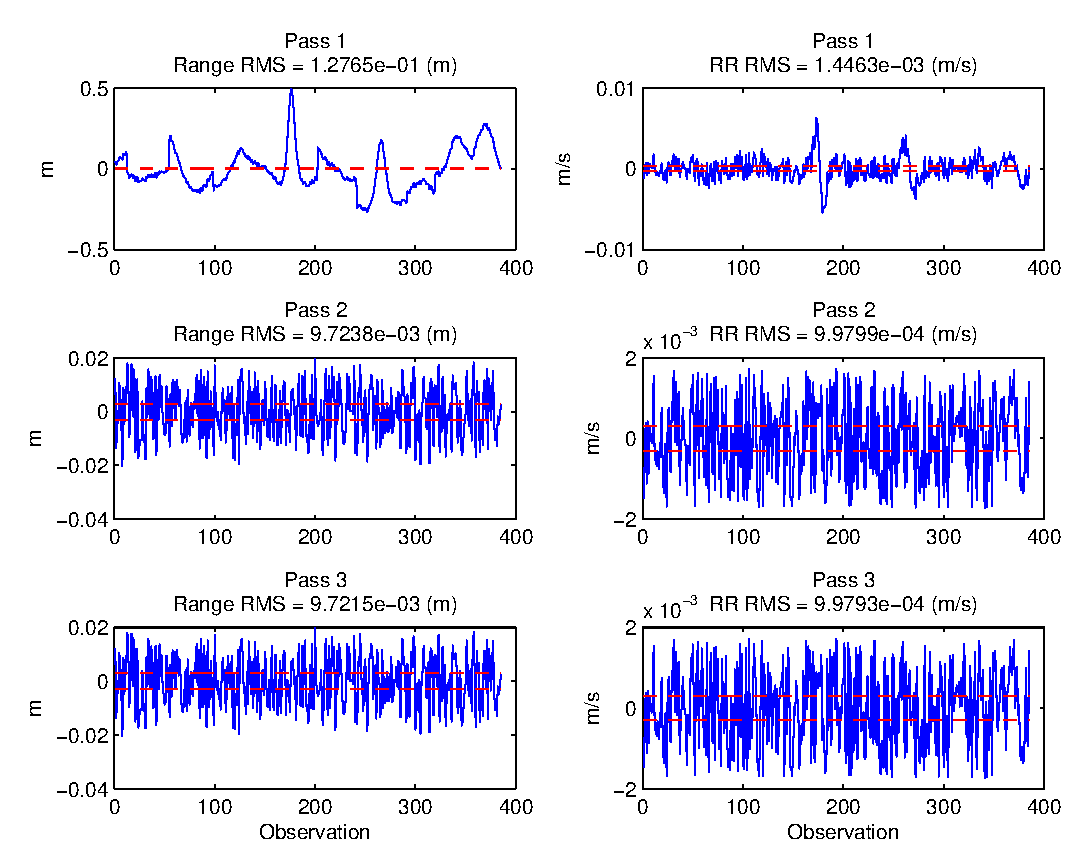
\includegraphics[width = 7cm]{DataNoise_dec_PFR.eps}
		}
		\subfigure[Decreased range noise variance]{
			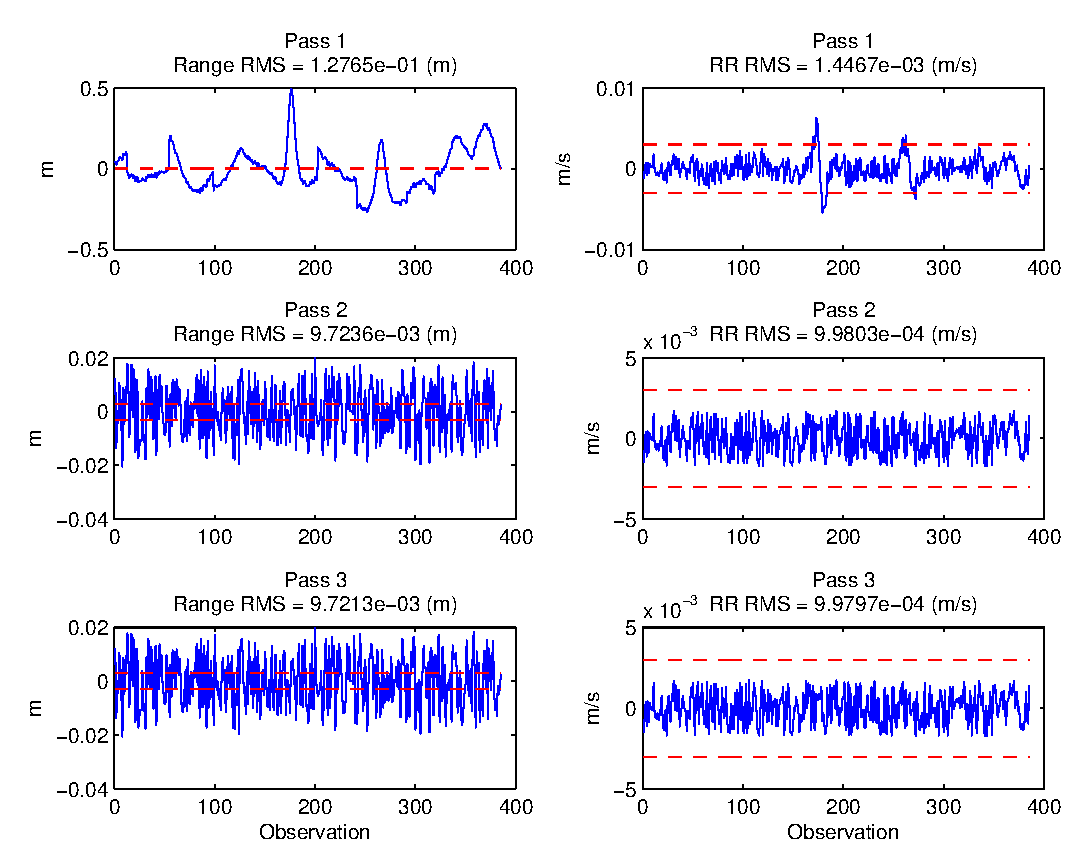
\includegraphics[width = 7cm]{DataNoise_rdec_PFR.eps}
		}
		\caption{Postfit residuals from varied data noise, batch algorithm. }
		\label{fig:Postfit_DN}
	\end{figure}	

	\begin{figure}[H]
		\centering
		\subfigure[Increased both noise variance]{
			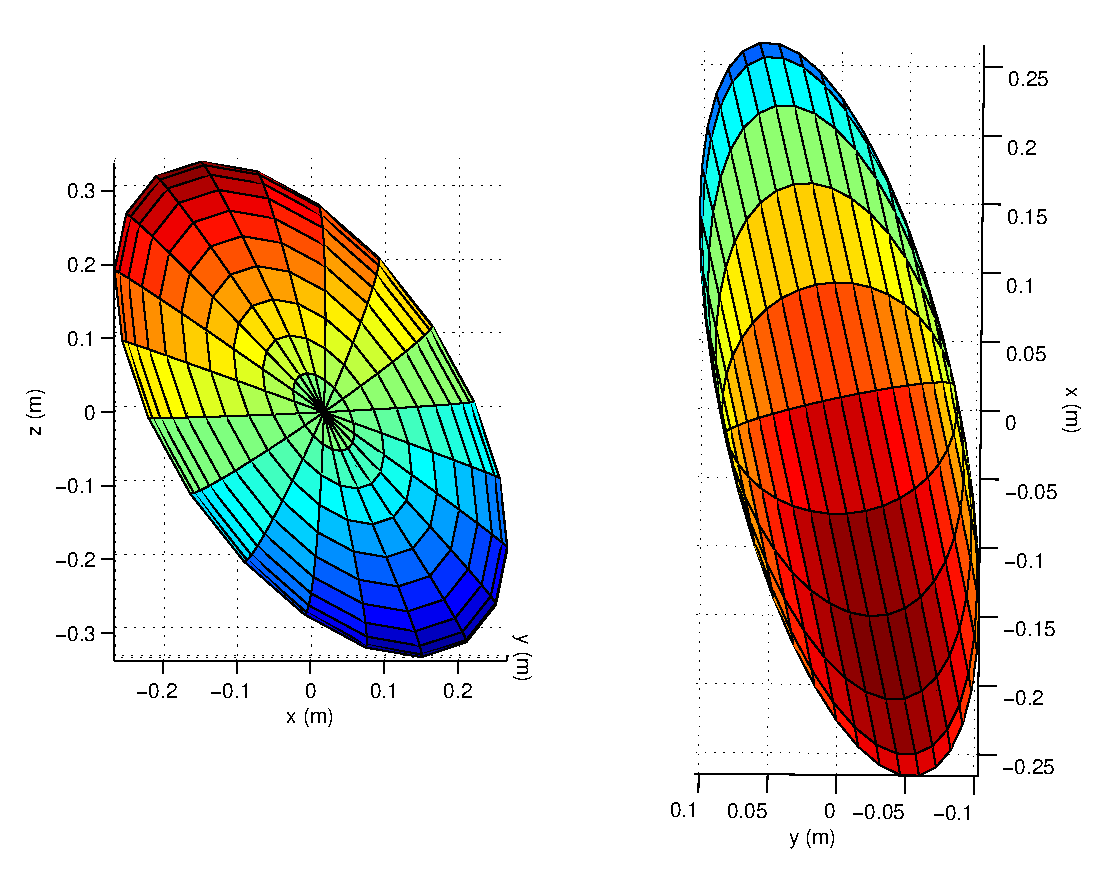
\includegraphics[width = 7cm]{DataNoise_inc_Ell.eps}
		}
		\subfigure[Decreased both noise variance]{
			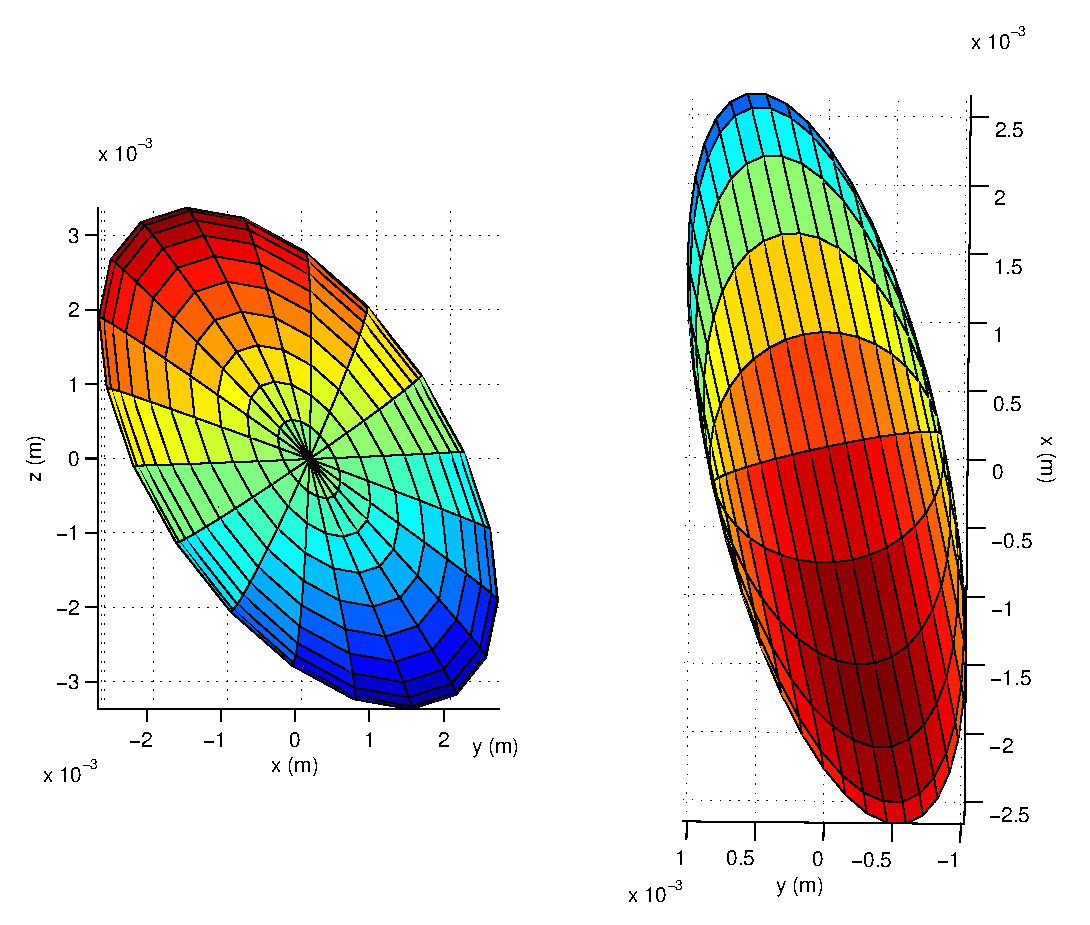
\includegraphics[width = 7cm]{DataNoise_dec_Ell.eps}
		}
		\subfigure[Decreased range noise variance]{
			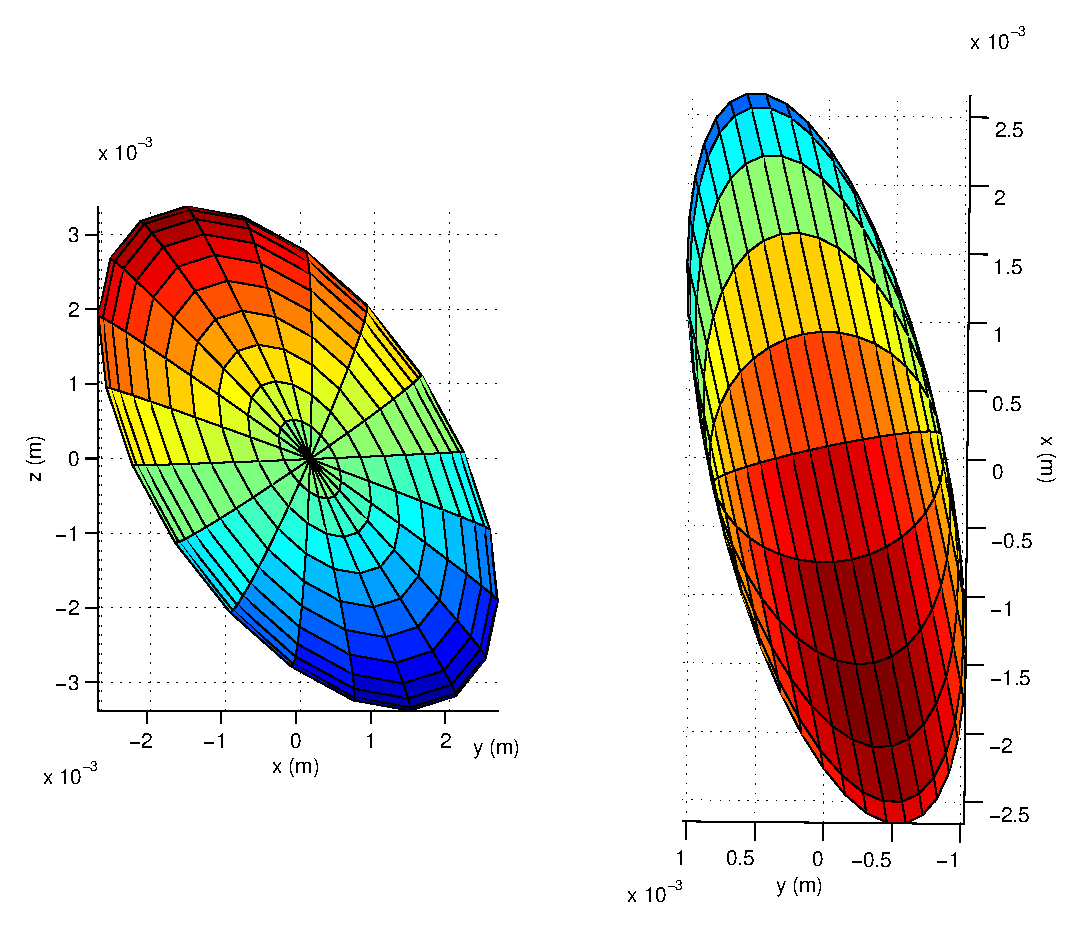
\includegraphics[width = 7cm]{DataNoise_rdec_Ell.eps}
		}
		\caption{3$\sigma$ error ellipsoids from varied data noise, batch algorithm. }
		\label{fig:ErrorEll_DN}
	\end{figure}	

	Changing both data noise variances only resulted in the measurement error envelopes changing; the RMS of the residuals stayed the same as before.  This was a result of Equation \ref{eq:BLS} and $W=R^{-1}$. $W$ is a weighting matrix that assigns more or less value on different measurement types at the same epoch.  Since the weights were changed by the same factor, the measurements had the same effect on the algorithm and the changes were cancelled out. The range-only change resulted in different final RMS values for the last pass of the batch algorithm.  The range-residual RMS decreased, while the range-rate-residual RMS increased. With a higher relative weighting compared to previous runs, the algorithm fit to the range data more than before, at the expense of the range-rate residuals.  Note: these noise variances were not changed in the data, which is why the noise in the residuals exceeds the error envelopes.  If the data noise actually changed, the residuals and RMS would change as well.
	
	\vspace{5 mm}

	The \textit{a priori} covariance for the satellite position and velocity were also varied: first they were squared from their original value, then set to 10 m\textsuperscript{2} and 25 m\textsuperscript{2}/s\textsuperscript{2} respectively.  The postfit residuals had the same RMS as the original case, and the relative differences between the cases were vanishingly small.  Looking to Equation \ref{eq:BLS_ap} showed why: \textit{a priori} data are treated like any other measurement.  As the number of measurements increase, the batch algorithm is less dependent on the \textit{a priori} information (as it would be for any single observation). Subtracting $\bar{P}_0^{-1}$ from the information matrix and $\bar{P}_0^{-1}\bar{\mathbf{x}}_0$ from the normal matrix had no noticeable effect on the matrices. This confirmed that there would be no appreciable change in the estimated position and velocity of the satellite. 

	\section{Conclusion and Recommendations}
	
	The batch processor, using Cholesky decomposition, had the best solution when looking at the residuals and error ellipsoid. Due to propagated errors and a collapsing covariance matrix, the CKF formulations all performed slightly worse.  The Potter formulation of the CKF fixed some of the residual outliers the other CKF formulations had. However, all CKF formulations succumbed to saturation.  The range measurements provided most of the confidence in the solution (when looking at the covariance), but the range-rate measurements were still useful in finding an estimate with a smaller standard deviation. Fixing of the Pacific site was crucial to the algorithms, as the batch processor only performed well when its position was well-known. Changing the variance of the data noise only had an effect when the weight ratio of the measurement types changed. Changing the \textit{a priori} state covariance had no affect on estimated position and velocity, since it was treated as one measurement among hundreds.
	
	\vspace{5 mm}

	From the results, a few areas of further research are recommended. First would be to determine the effect of azimuth and elevation measurements from the sites.  This might improve measurement geometry, and not require the Pacific site to be fixed as it was.  Next would be to include process noise in an attempt to thwart filter divergence in the CKF.  Finally, EKF results may perform better than the CKF if it were implemented.
	
	\vspace{5 mm}

	There were a few trade-offs identified when considering which algorithm to implement for a given situation.  The batch agorithm is built for post-processing, not ideal for autonomous navigation.  The CKF can process measurements sequentially, which would be good for autonomous navigation.  However,  filter saturation can happen if the CKF has too small a covariance. The Joseph and Potter formulations each use more computations, and thus more CPU load.  Modern computers can handle such things in realtime, but radiation-resistant/hardened computers for space applications may not be able to. 
	
	\vspace{5 mm}

	This project made me aware of several ways that estimation can be performed and improved.  I would have liked to see how process noise and the EKF would affect my solutions, but time at the end of this semester was a valuable resource (for everyone, I'm sure).  The project format was also good because it allowed a lot of time to explore, compared to homeworks.  My recommendation would be to include azimuth/elevation data, perhaps, to see the effect on ground site geometry.
		
	
	\begin{thebibliography}{9}% maximum number of references (for label width)
		\bibitem{Born} 
		\noindent Born, G., Schutz, B., and Tapley, B. \emph{Statistical Orbit Determination}, Elsevier Academic Press, 2004.
		
		
	\end{thebibliography}
	
	\newpage

	\section{Appendix A: Supplemental Data}
	\noindent This appendix contains data to further support the conclusions drawn previously.

	\begin{table}[H]% no placement specified: defaults to here, top, bottom, page
		\begin{center}
			\caption{Effects of ground sites being fixed: percent differences with Pacific site fixed.}
			\label{t:GSFixed}
			\begin{tabular}{c|c|c|c|c|c|c}
\hline & Init. State & Init. State &  Init. State & Final State & Final State & Final State \\
 &None Fixed & Turk. Fixed &  Gnld Fixed & None Fixed & Turk. Fixed & Gnld Fixed\\ 
Element & \%-Diff & \%-Diff & \%-Diff & \%-Diff & \%-Diff & \%-Diff \\ \hline
$x$         &    621.2236e-006 &    2.0129e-003 &    1.4113e-003 &  360.0386e-006 &    1.4995e-003 &    1.0444e-003 \\
$y$         &     13.1088e-006 &    7.1406e-006 &   25.0578e-006 &   12.7798e-006 &   55.9252e-006 &   55.3506e-006 \\
$z$         &     12.9819e-009 &  162.5944e-006 &   45.6413e-006 &   60.3596e-009 &  144.1028e-006 &   68.4470e-006 \\
$\dot{x}$   &    190.4063e-006 &  705.3215e-006 &  623.0584e-006 &  120.1942e-006 &  639.2765e-006 &  632.2569e-006 \\
$\dot{y}$   &     42.5877e-006 &  219.2785e-006 &  197.9999e-006 &   38.2558e-006 &  221.0029e-006 &  111.4226e-006 \\
$\dot{z}$   &     28.6739e-009 &   86.5533e-006 &   32.7989e-006 &    2.4637e-009 &   26.4105e-006 &   35.9176e-006 \\
$\mu$       &     13.8104e-006 &  175.0525e-006 &    6.2032e-006 &   13.8493e-006 &  132.0406e-006 &    6.4772e-006 \\
$J_2$       &      2.0694e-003 &    4.6110e-003 &    6.9971e-003 &    2.0742e-003 &    3.7851e-003 &    4.8352e-003 \\
$C_D$       &      1.5264e+000 &   22.0637e+000 &    2.3791e+000 &    1.6609e+000 &   19.1942e+000 &    1.9327e+000 \\
$X_{site1}$ &    117.9602e-006 &  804.1027e-006 &  796.4735e-006 &   67.8348e-006 &  601.9432e-006 &  607.2670e-006 \\
$Y_{site1}$ &    175.8016e-006 &    1.5927e-003 &    1.3662e-003 &   84.1457e-006 &    1.1994e-003 &    1.0358e-003 \\
$Z_{site1}$ &    126.4290e+009 &    1.1550e+012 &  629.9792e+009 &  275.2865e+009 &    1.9193e+012 &    1.0408e+012 \\
$X_{site2}$ &    110.5614e-006 &    1.0513e-003 &  720.7838e-006 &   53.6770e-006 &  792.0839e-006 &  549.5881e-006 \\
$Y_{site2}$ &    148.7567e-006 &    1.2350e-003 &  907.0205e-006 &   67.8854e-006 &  926.0770e-006 &  691.1627e-006 \\
$Z_{site2}$ &     13.7672e-006 &  608.6156e-006 &   12.5391e-006 &   13.8041e-006 &  455.2844e-006 &    8.4452e-006 \\
$X_{site3}$ &    353.8359e-006 &    3.9967e-003 &    3.7872e-003 &  183.4620e-006 &    3.0113e-003 &    2.8756e-003 \\
$Y_{site3}$ &     26.0506e-006 &  327.3688e-006 &  609.0337e-006 &    1.0045e-006 &  250.4703e-006 &  462.6257e-006 \\
$Z_{site3}$ &     28.7080e-006 &  383.3949e-006 &  168.8545e-006 &   28.7864e-006 &  290.1459e-006 &  120.7160e-006 \\

			\end{tabular}
		\end{center}
	\end{table}  
	
	\begin{table}[H]% no placement specified: defaults to here, top, bottom, page
		\begin{center}
			\caption{Effects of ground sites being fixed: percent differences with Pacific site fixed.}
			\label{t:Potter_results}
			\begin{tabular}{c|c}
\hline & Final State  \\
 &CKF-Potter \\ 
Element & \%-Diff  \\ \hline
$x$         &     21.6987e-006 \\
$y$         &      1.1305e-006 \\
$z$         &     18.4758e-006 \\
$\dot{x}$   &     45.0495e-006 \\
$\dot{y}$   &     11.8521e-006 \\
$\dot{z}$   &      5.2066e-006 \\
$\mu$       &     21.4489e-006 \\
$J_2$       &    116.1292e-003 \\
$C_D$       &     14.8210e+000 \\
$X_{site1}$ &     36.4355e-012 \\
$Y_{site1}$ &     36.4389e-012 \\
$Z_{site1}$ &     37.6443e+003 \\
$X_{site2}$ &    518.4772e-006 \\
$Y_{site2}$ &    617.8071e-006 \\
$Z_{site2}$ &    306.6402e-006 \\
$X_{site3}$ &      1.8233e-003 \\
$Y_{site3}$ &    292.8506e-006 \\
$Z_{site3}$ &     96.2513e-006 \\

			\end{tabular}
		\end{center}
	\end{table}  
	

	\newpage

	\section{Appendix B: Code}

This appendix contains all Matlab code created by the author for the project.

%    \section{Appendix B}
%This appendix contains all Matlab code used by the authors to analyize their data.
%    
%    \lstset{language=Matlab,%
%    	%basicstyle=\color{red},
%    	breaklines=true,%
%    	morekeywords={matlab2tikz},
%    	keywordstyle=\color{blue},%
%    	morekeywords=[2]{1}, keywordstyle=[2]{\color{black}},
%    	identifierstyle=\color{black},%
%    	stringstyle=\color{mylilas},
%    	commentstyle=\color{mygreen},%
%    	showstringspaces=false,%without this there will be a symbol in the places where there is a space
%    	numbers=left,%
%    	numberstyle={\tiny \color{black}},% size of the numbers
%    	numbersep=9pt, % this defines how far the numbers are from the text
%    	emph=[1]{for,end,break},emphstyle=[1]\color{red}, %some words to emphasise
%    	%emph=[2]{word1,word2}, emphstyle=[2]{style},   
%    }
    
%    \lstinputlisting{ASEN5090_ecef2azelrange.m}
%    \vspace{5mm}
%    
%    \lstinputlisting{ASEN5090_GPSvis.m}
%    \vspace{5mm}
%\lstinputlisting{HW5_rel_err.m}
%\vspace{5mm}
%\lstinputlisting{import_gps_data.m}
%\vspace{5mm}
%\lstinputlisting{datenum8601.m}
%\vspace{5mm}
%\lstinputlisting{lab_err_plots.m}
%\vspace{5mm}
	
\end{document}

% - Release $Name:  $ -
